%Khwopa college of Engineering Latex Template
%Prepared by Mukesh Kumar Pokharel for Project Proposal as references.

\documentclass[12pt, a4paper, oneside, openany]{report}

% ── Encoding ──────────────────────────────────────────────────────────────────
\usepackage[utf8]{inputenc}

% ── Page Layout ───────────────────────────────────────────────────────────────
\usepackage[left=1.2in, right=1in, top=1.2in, bottom=1in, 
            headheight=6pt, a4paper]{geometry}

% ── Graphics & Figures ────────────────────────────────────────────────────────
\usepackage{graphicx}
\usepackage{subcaption}
\usepackage{float}

% ── Math ──────────────────────────────────────────────────────────────────────
\usepackage{amsmath, amssymb, amsfonts}
\usepackage{setspace}

% ── Tables ────────────────────────────────────────────────────────────────────
\usepackage{array}
\usepackage{longtable}

% ── Text & Formatting ─────────────────────────────────────────────────────────
\usepackage{ragged2e}
\usepackage{lipsum}
\usepackage{emptypage}
\let\cleardoublepage\clearpage 
\usepackage{placeins}
\setlength{\parskip}{0pt}
\renewcommand{\baselinestretch}{1.5}
\raggedbottom
\usepackage{cleveref}

% ── Bibliography ──────────────────────────────────────────────────────────────
\usepackage{cite}

% ── Section Title Formatting ──────────────────────────────────────────────────
\usepackage{titlesec}

\titleformat{\chapter}[display]
    {\centering\normalfont\large\bfseries}
    {\MakeUppercase{\chaptertitlename} \thechapter}{2pt}{\Large}
\titlespacing{\chapter}{0pt}{0pt}{4pt}

\titleformat{\section}
    {\normalfont\large\bfseries}{\thesection}{1em}{}

\titleformat{\subsection}
    {\normalfont\normalsize\bfseries}{\thesubsection}{1em}{}

\titleformat{\subsubsection}
    {\normalfont\normalsize\bfseries}{\thesubsubsection}{1em}{}

% ── TOC Depth ─────────────────────────────────────────────────────────────────
\setcounter{tocdepth}{3}
\setcounter{secnumdepth}{3}

% ── Hyperref LAST — removes red boxes, enables clickable TOC ──────────────────
\usepackage{hyperref}
\hypersetup{
    colorlinks=false,
    pdfborder={0 0 0},
    linkbordercolor={0 0 0},
    citebordercolor={0 0 0},
    urlbordercolor={0 0 0}
}

% ══════════════════════════════════════════════════════════════════════════════
\begin{document}
\noindent
\let\cleardoublepage\clearpage

    % ── Front Matter ──────────────────────────────────────────────────────────
    \thispagestyle{empty}
\singlespacing
 \begin{center}
		\thispagestyle{empty}
		\Large\textbf{TRIBHUVAN UNIVERSITY}\\
		\Large\textbf{INSTITUTE OF ENGINEERING }\\
		\vspace{0.2in}
		\large{\textbf{Khwopa College Of Engineering}\\}
		\normalsize{Libali, Bhaktapur\\}
		\large\textbf{Department of Computer and Electronics Engineering}
		\vspace{0.2in}
		\begin{figure}[h]
		    \centering
			    
\includegraphics[width=0.25\textwidth]{img/Khwopalogo.jpg}
		\end{figure}
		
		\vspace{0.2in}
		\large{A FINAL REPORT ON\\\textbf{Nepali Handwritten Word Digitization Using Transformer Model}\\}
		
		\vspace{0.2in}
		\large{\textit{Submitted in partial fulfillment of the requirements for the degree in Bachelor of Computer Engineering\\}}
		
		
		%\large{\textbf{BACHELOR OF COMPUTER ENGINEERING}\\}
		
		\vspace{0.2in}
		\large{Submitted by}\\
		\begin{tabular}{p{3.5in}p{3in}}
        %Write name in alphabetical order
    
       \hspace{0.3cm}Anjila Dangol& KCE079BCT010\\
        \hspace{0.3cm}Arpita Rimal & KCE079BCT012\\
        \hspace{0.3cm}Ayusha Shrestha & KCE079BCT017\\
        \hspace{0.3cm}Sneha Chaulagain & KCE079BCT042\\
		 \vspace{0.2in}
		\end{tabular}
		%\vspace{1cm}
		\large\textbf{Under the Supervision of}\\[0.1cm]
      \normalsize{Er.Anish Shilpakar}\\
      \normalsize{Data Engineer}\\
      \normalsize{Leapfrog Technology}\\[0.4cm]
		%	\vspace{1cm}
			\vspace{2cm}
		\large{\textbf{Khwopa College of Engineering}\\}
			\normalsize{Libali, Bhaktapur\\
			April,2026
		}
    \end{center}
\onehalfspacing
    \newgeometry{top=1in}
\pagenumbering{gobble}
\vspace*{1.3in}
\begin{center}
\large{\textbf{CERTIFICATE OF APPROVAL}}
\end{center}
\vspace{1cm}

\noindent
This is to certify that this minor project work entitled \textbf{``Nepali Handwritten Word Digitization Using Transformer Model''}, submitted by Anjila Dangol (KCE079BCT010), Arpita Rimal (KCE079BCT012), Ayusha Shrestha (KCE079BCT017) and Sneha Chaulagain (KCE079BCT042) has been examined and accepted as the partial fulfillment of the requirements for the degree of Bachelor in Computer Engineering. The project was carried out under special supervision and within the time frame prescribed by the syllabus.

\vspace{2cm}

\noindent
\begin{minipage}[t]{0.45\textwidth}
\centering
..........................................\\
\textbf{Er. Pratik Timalshena} \\
External Examiner \\
Senior Lecturer \\
Department of Electronics and \\
Computer Engineering \\
Sagarmatha Engineering College
\end{minipage}
\hfill
\begin{minipage}[t]{0.45\textwidth}
\centering
..........................................\\
\textbf{Er. Anish Shilpakar} \\
Project Supervisor \\
Data Engineer \\
Leapfrog Technology
\end{minipage}

\vspace{1.5cm}

\vspace{0.5cm}
\begin{center}
..........................................\\
\textbf{Er. Dinesh Gothe}\\
Head of Department\\
Department of Computer and Electronics Engineering\\
Khwopa College of Engineering
\end{center}
\newpage

\pagenumbering{roman}
\addcontentsline{toc}{section}{Copyright}
\begin{center}
    {\Large\bfseries COPYRIGHT\copyright}
\end{center}
\vspace{1em}
\normalsize
\justify
The author has agreed that the library of Khwopa College of Engineering may make this report freely available for inspection. Moreover, the author has agreed that permission for extensive copying of this project report for scholarly purposes may be granted by the supervisor who supervised the project work recorded herein or, in their absence, by the Head of the Department where the project report was completed. It is understood that recognition will be given to the author of the report and to the Department of Computer and Electronics Engineering, KhCE, for any use of the material in this project report. Copying, publication, or any other use of this report for financial gain without the approval of the department and the author's written permission is prohibited. Requests for permission to copy or make any other use of the material in this report, in whole or in part, should be addressed to:

\vspace{1.5cm}
\noindent\textbf{Head of Department} \\
Department of Computer and Electronics Engineering \\
Khwopa College of Engineering (KhCE) \\
Libali-08, Bhaktapur, Nepal
\newpage

\addcontentsline{toc}{section}{Acknowledgement}
\begin{center}
    {\Large\bfseries ACKNOWLEDGEMENT}
\end{center}
\vspace{1.2cm}
\normalsize
\noindent
We would like to express our deepest gratitude to our supervisor of the project, \textbf{Er.Anish Shilpakar}, for his immense support and guidance throughout the course of this project. His insightful advice, expertise, and unwavering support have been crucial to our work's successful completion. This project would not have been possible without his guidance and mentorship.

\noindent We would also like to extend gratitude to our teachers \textbf{Er.Mukesh Kumar Pokharel} and \textbf{Er.Anish Baral} for their constructive feedback and unwavering support throughout the project. The expertise and analytical recommendations gave us fresh viewpoints, which were crucial for improving our project.

\noindent A special thanks to \textbf{Er.Dinesh Gothe} for his encouragement and assistance. We have been greatly inspired by his encouragement, which has kept us dedicated and focused on the project.

\noindent Furthermore, we are grateful to our institution faculty members, and peers for providing us with the necessary resources, facilities, and a conducive learning environment that greatly contributed to our work.

\noindent Finally, we would like to thank everyone who has directly or indirectly assisted us in initiation of our project.

\vspace{1.5cm}
\begin{tabular}{l@{\hspace{3cm}}l}
Anjila Dangol      & KCE079BCT010 \\
Arpita Rimal       & KCE079BCT012 \\
Ayusha Shrestha    & KCE079BCT017 \\
Sneha Chaulagain   & KCE079BCT042 \\
\end{tabular}
\newpage

\addcontentsline{toc}{section}{Abstract}
\begin{center}
    {\Large\bfseries ABSTRACT}
\end{center}
\vspace{1em}
\normalsize
\noindent
Devanagari is the primary script used for writing the Nepali language and contains complex character structures, conjunct consonants, and vowel modifiers that make handwritten text recognition a challenging task. This project aims to develop a Transformer-based Optical Character Recognition (OCR) system for recognizing handwritten Nepali words and converting them into digital text.The proposed system adopts a TrOCR-inspired architecture that combines a pretrained Vision Transformer (ViT) encoder with a lightweight custom BERT-based Transformer decoder. The ViT encoder extracts contextual visual representations from handwritten word images, while the decoder, designed with a compact Transformer configuration and cross-attention mechanism, generates the corresponding Nepali word sequence in Unicode format. Both components are integrated using HuggingFace's VisionEncoderDecoderModel framework to enable end-to-end handwritten word recognition.Experimental results demonstrate that the proposed model achieves a Character Error Rate (CER) of 5.43\%, a Word Error Rate (WER) of 16.58\%, and an overall accuracy of 83.42\%, indicating its effectiveness in recognizing complex handwritten Nepali text. The developed system provides a promising approach for digitizing handwritten Nepali documents and supports the preservation and accessibility of Nepali written resources.

\vspace{1em}
\noindent
\textbf{Keywords}: \textit{Nepali Handwritten Word Recognition, Optical Character Recognition, Vision Transformer encoder, TrOCR, BERT, Devanagari Script.}
\newpage

\tableofcontents
\newpage

\addcontentsline{toc}{section}{List of tables}
\listoftables
\newpage

\addcontentsline{toc}{section}{List of figures}
\listoffigures
\newpage
\addcontentsline{toc}{section}{List of Symbols and Abbreviation}
\begin{center}
    {\Large\bfseries List of Symbols and Abbreviation}
\end{center}
\vspace{0.5em}
\setstretch{1.2}
\noindent\begin{tabular}{ll}
\hline
\textbf{Abbreviation} & \textbf{Full Form} \\
\hline
AdamW   & Adaptive Moment Estimation with Weight Decay \\
AI      & Artificial Intelligence \\
BERT    & Bidirectional Encoder Representations from Transformers \\
BiLSTM  & Bidirectional Long Short-Term Memory \\
BOS     & Beginning of Sequence \\
CER     & Character Error Rate \\
CLS     & Classification Token \\
CNN     & Convolutional Neural Network \\
CTC     & Connectionist Temporal Classification \\
CUDA    & Compute Unified Device Architecture \\
EOS     & End of Sequence \\
FFN     & Feedforward Neural Network \\
fp16    & 16-bit Floating Point \\
GELU    & Gaussian Error Linear Unit \\
GPU     & Graphics Processing Unit \\
HTR     & Handwritten Text Recognition \\
HWR     & Handwritten Word Recognition \\
IIIT    & International Institute of Information Technology \\
LSTM    & Long Short-Term Memory \\
MHA     & Multi-Head Attention \\
ML      & Machine Learning \\
NED     & Normalized Edit Distance \\
NFC     & Unicode Normalization Form C \\
NHWDTM  & Nepali Handwritten Word Digitization Using Transformer Model \\
OCR     & Optical Character Recognition \\
ReLU    & Rectified Linear Unit \\
RNN     & Recurrent Neural Network \\
SDLC    & Software Development Lifecycle \\
SVM     & Support Vector Machines \\
TrOCR   & Transformer-based Optical Character Recognition \\
TTA     & Test-Time Augmentation \\
UI      & User Interface \\
ViT     & Vision Transformer \\
WER     & Word Error Rate \\
\hline
\end{tabular}


    % ── Chapters ──────────────────────────────────────────────────────────────
    \chapter{INTRODUCTION}
        \pagenumbering{arabic}
        \section{Background Introduction}


Handwritten text recognition (HTR) has gained significant attention in recent years due to its wide applications in document digitization, archival preservation, and human--computer interaction. Despite notable progress in optical character recognition (OCR) for printed text, recognizing handwritten scripts remains a challenging problem, particularly for complex writing systems such as Devanagari.

\noindent Devanagari, the script used for the Nepali language and several other South Asian languages, exhibits high structural complexity. It consists of base characters, vowel modifiers (matras), conjunct consonants, and compound symbols formed by combining multiple glyphs into a single unit. This complexity is further amplified in handwritten form due to variations in individual writing styles, cursive connections, distortions, and inconsistent spacing between characters and words. These characteristics make segmentation and recognition tasks significantly more difficult compared to Latin-based scripts.

\noindent Existing handwritten word recognition (HWR) systems for Nepali and Devanagari scripts have primarily relied on handcrafted feature extraction methods or convolutional neural networks (CNNs) \cite{baral2019handwritten, ghimire2020nepali, acharya2022nepali}. While CNN-based approaches have shown promising results in capturing local spatial features, they often struggle to model long-range dependencies and sequential context within text, which are crucial for accurate word-level recognition \cite{michael2019evaluating}. Furthermore, the scarcity of large-scale, diverse, and publicly available Nepali handwriting datasets limits the generalization capability and robustness of these models \cite{10.1007/978-3-030-86337-1_30}.

\noindent Recent advances in deep learning, particularly Transformer-based architectures, have demonstrated superior performance in various vision and sequence modeling tasks. Vision Transformers (ViT) \cite{dosovitskiy2020image} and Transformer-based OCR models such as TrOCR \cite{li2023trocr} have shown strong capability in capturing global contextual relationships within images, making them well-suited for handwritten text recognition. Several recent studies have explored the application of Transformers for Indic scripts and multilingual OCR tasks, reporting improved accuracy over traditional CNN-based approaches.\cite{hasan2023optical, li2025htr,10.1007/978-3-031-93688-3_17}.

\noindent These developments highlight the need for more robust and context-aware models for handwritten Nepali word recognition and digitization. In this work, we explore the use of Transformer-based Optical Character Recognization (TrOCR)-based architectures to effectively capture both visual features and contextual dependencies, aiming to improve performance for handwritten Nepali text and their digitization.


        \section{Motivation}
Recognizing handwritten Nepali text is challenging due to the complexity of the Devanagari script, which includes compound characters, vowel diacritics, and cursive variations. Manual digitization is time-consuming and error-prone, while existing systems based on handcrafted features or CNNs often fail to capture long-range dependencies and contextual relationships. Limited availability of large, diverse Nepali handwriting datasets further restricts model performance. Recent advances in Transformer-based architectures, such as TrOCR, provide an opportunity to develop an end-to-end system that can accurately recognize handwritten Nepali words, supporting efficient digitization and preservation of Nepali textual resources.

        \section{Problem Statement}
Nepali handwritten word recognition using Transformer-based models faces several key challenges:

\begin{itemize}
    \item \textbf{Structural complexity:} The Devanagari script contains conjunct consonants, vowel modifiers, and compound characters, making recognition difficult \cite{baral2019handwritten,ghimire2020nepali}.
    
    \item \textbf{Handwriting variation:} Diverse writing styles reduce segmentation and recognition accuracy \cite{michael2019evaluating}.
    
    \item \textbf{Limitations of existing methods:} CNN and handcrafted approaches capture local features but fail to model long-range dependencies and sequence context effectively \cite{dosovitskiy2020image,li2023trocr}.
    
    \item \textbf{Limited datasets:} A lack of large and diverse Nepali handwriting datasets restricts generalization \cite{10.1007/978-3-030-86337-1_30,anand2023devanagari,rajak_indic_data}.
\end{itemize}

Although Transformer-based OCR models like TrOCR and Vision Transformers improve global context learning, they still struggle with the linguistic complexity of Nepali handwritten text, highlighting the need for a robust end-to-end OCR system in Unicode format \cite{hasan2023optical,parres2023fine,li2025htr}.
%         \section{Problem Statement}
% \begin{itemize}
%     \item Handwritten Nepali word recognition is challenging due to the complex Devanagari script, which includes conjunct consonants, vowel modifiers, and variations in individual handwriting styles \cite{baral2019handwritten,ghimire2020nepali}.
%     \item Existing systems based on CNNs or handcrafted features struggle to capture long-range dependencies and sequential context, and the lack of large, diverse Nepali handwriting datasets limits model accuracy and generalization \cite{hasan2023optical,li2023trocr}.
% \end{itemize}

      \section{Objective} 
The main objective of this project is:
\begin{itemize}
    \item To design and develop a Transformer-based OCR system that accurately recognizes and digitizes handwritten Nepali words in the Devanagari script.
\end{itemize}

\section{Scope of Project}
The scope of this project includes:
\begin{itemize}
    \item Developing an end-to-end Transformer-based OCR system for recognition of handwritten Nepali words in Devanagari script.
    \item Enhancing model generalization to handle diverse handwriting styles, complex conjunct consonants, and compound characters.
    \item Facilitating digitization, preservation, and accessibility of handwritten Nepali documents for educational, cultural, and research purposes.
\end{itemize}
        %\section{Organization of project}
    
    
    \chapter{LITERATURE REVIEW}

\section{Literature Review}

\noindent The area of Handwritten Text Recognition (HTR) has witnessed an enormous shift from the tedious process of manual feature engineering to the era of deep learning, and now, to the era of advanced Transformer-based models. Initial attempts in digitizing Nepali handwriting scripts often encountered roadblocks due to the script's structural complexities. Dense compound character sets, floating vowel modifiers (matras), and the highly unpredictable nature of cursive handwriting are some of the challenges.

\noindent A significant milestone was reached with the advent of Convolutional Neural Networks (CNNs), as these networks are capable of learning and extracting such complex features \cite{baral2019handwritten, ghimire2020nepali, acharya2022nepali}. Although CNNs proved to be highly efficient in recognizing individual spatial patterns, they faced a structural limitation in incorporating the sequential patterns and long-range dependencies necessary for smooth reading of connected words. This, in turn, led to the natural progression toward sequence-to-sequence models and, consequently, Transformers. Using the self-attention mechanism, Transformers are able to bypass the need for a recurrent structure, as they can consider the entire context of a word. In fact, Vision Transformers and TrOCR models are currently achieving state-of-the-art results, proving to be highly efficient in modeling the complex visual geometry of low-resource languages like Nepali \cite{li2023trocr, hasan2023optical, li2025htr}.

\subsection{CNN-based Handwriting Recognition}
CNNs were undoubtedly a huge step forward for HTR, as they circumvented the need for feature extraction and instead learned hierarchical spatial features on their own. For example, Baral had built a good foundation with a CNN-based system that was specifically designed for isolated word recognition in Nepali scripts \cite{baral2019handwritten}. Ghimire et al. had also further improved this by optimizing the preprocessing steps to be better suited for handling Devanagari scripts \cite{ghimire2020nepali}, and Acharya et al. had also used similar CNN approaches for converting handwritten Nepali scripts to digital text \cite{acharya2022nepali}. However, there was a catch. While these models were extremely effective for isolated word recognition, standard CNNs did not possess the ``memory" that is often required for handling global dependencies in connected handwriting. This meant that it was extremely sensitive to the stylistic variations in handwriting.

\subsection{Sequence Modeling and Indic Script OCR}
To overcome the blind spots of CNNs on the word level, naturally, the solution was to resort to sequence modeling. For instance, Michael et al. demonstrated how important sequence-to-sequence models can be in cases where you have to directly map unsegmented image data to output text \cite{michael2019evaluating}.

\noindent When we consider the Indic scripts in more detail, the early Nepali-based OCR systems heavily relied on hybrid approaches that combined template matching and feature extraction. However, these were perfectly adequate for simple and well-structured characters but failed miserably when it came to the complex and non-uniform compound characters. The greatest barrier to deeper sequential learning was the absence of data. Gongidi and Jawahar alleviated this problem to some extent by introducing the IIIT-HW-Dev dataset and providing the long-awaited benchmark for Devanagari word-level OCR \cite{10.1007/978-3-030-86337-1_30}. Following this, Lalitha et al. attempted to explore new approaches that could improve the accuracy of Indic HTR systems, further supporting the claim that cursive Devanagari needs highly robust models \cite{10.1007/978-3-031-93688-3_17}.

\subsection{Vision Transformers for Handwritten Text}
Transformers have revolutionized the way we think about handwriting recognition. They have rewritten the rules. It began with Dosovitskiy et al.'s \cite{dosovitskiy2020image} Vision Transformer (ViT) model, which showed it is possible to process image patches with self-attention mechanisms and achieve superior performance compared to traditional convolutional networks. This is something we have seen being applied in handwriting recognition. In fact, Parres and Paredes \cite{parres2023fine} used vision-based encoder-decoder models to recognize complex, cursive scripts in historical documents. On the other hand, Yajima et al. \cite{yajima2024text} used Vision Transformers to recognize text in images and also classify script styles. More recently, Li et al. \cite{li2025htr} took it to another level with HTR-VT, which uses Vision Transformers in conjunction with sharpness-aware minimization to achieve state-of-the-art performance. In fact, across the board, comprehensive reviews of handwriting recognition models \cite{article} indicate that Transformer models are the new gold standard in extracting text from images.

\subsection{TrOCR and End-to-End Recognition}
A pivotal innovation in the field is the development of TrOCR by Li et al.~\cite{li2023trocr}. This architecture utilizes pre-trained models for both image and text modalities in an end-to-end fashion. The significance of TrOCR lies in its removal of complex CNN backbones and the reliance on Connectionist Temporal Classification (CTC) loss functions, opting instead for pure self-attention and cross-attention mechanisms. The flexibility of this model has been demonstrated in diverse applications, such as the handwriting pattern recognition research conducted by Adeli Shamsabad and Suen~\cite{inproceedings}. 

\noindent For low-resource languages, Hasan et al. proposed a Transformer-based model specifically designed for Nepali and Bengali OCR, achieving significant accuracy improvements with a reported Word Error Rate (WER) of 0.15~\cite{hasan2023optical}. Despite these strides, a notable research gap remains in the adoption of highly compressed, localized TrOCR variants. Specifically, the integration of a custom, lightweight BERT-based decoder engineered to address the unique phonetic and morphological nuances of the Devanagari script has yet to be fully explored for the Nepali language. This study seeks to address this gap.

\subsection{Role of Language Models and Custom Decoders in HTR}
While Vision Transformers excel at extracting spatial and structural features from word images, the ultimate accuracy of an end-to-end HTR system is heavily dependent on the decoder's capacity for sequence modeling~\cite{michael2019evaluating}. In TrOCR-style architectures, the decoder functions as a language model, generating character sequences based on visual embeddings and the linguistic context of the target language~\cite{li2023trocr}. Standard TrOCR implementations often utilize pre-trained English models like RoBERTa, which may not adequately capture the complexities of Indic scripts.

\noindent In the Devanagari script, relying exclusively on visual features can result in ambiguity, particularly when distinguishing between visually similar characters or tightly packed conjuncts~\cite{ghimire2020nepali}. By employing a localized, script-specific language model such as a custom-configured BERT decoder, it is possible to leverage the statistical probability of character co-occurrence in Nepali. Fine-tuning such a decoder specifically for Devanagari text~\cite{hasan2023optical, 10.1007/978-3-030-86337-1_30} provides the linguistic intuition necessary to correct visual misclassifications, representing a critical optimization pathway that this project investigates.

\newpage

\section{Related Theories}
\subsection{Optical Character Recognition (OCR)}

OCR is a technology that detects and converts printed or handwritten text found in digital images into machine-encoded, editable text. OCR systems combine hardware and software to transform physical documents into formats that computers can process and search. The most widely known application of OCR
is converting scanned paper documents into editable word-processor files. Modern OCR pipelines typically consist of four stages: image acquisition,preprocessing, character or word recognition, and post-processing. Handwritten text recognition is a particularly challenging subfield of OCR because writing
styles, stroke widths, and character spacing vary enormously across individuals.

\begin{figure}[h]
  \centering
  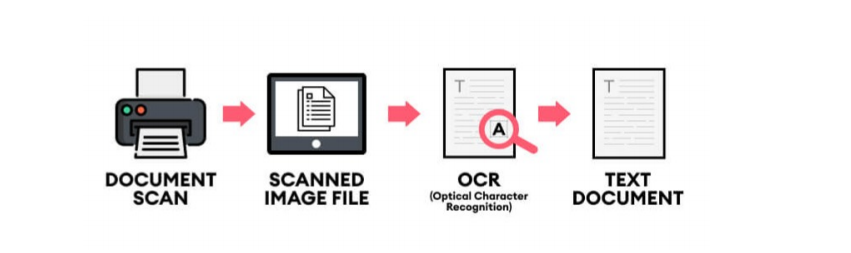
\includegraphics[width=0.75\textwidth]{img/ocr.png}
  \caption{General OCR Pipeline}
  \label{fig:ocr}
\end{figure}

\subsection{Traditional Approaches to OCR}

\subsubsection{Matrix Matching}
Matrix Matching was one of the earliest techniques used in OCR systems. An input character image is partitioned into a fixed grid and each cell is mapped to a pixel value, forming a matrix. This matrix is then compared against a library of pre-stored character templates using a similarity measure.While effective for clean, uniformly typeset text, matrix matching degrades sharply when character fonts, sizes, or orientations deviate from the stored templates, making it unsuitable for handwritten scripts such as Devanagari.

\subsubsection{Structural and Feature-Based Methods}
Structural analysis methods decompose a character into its constituent strokes,loops, junctions, and endpoints. Recognition is achieved by matching thesestructural primitives against a grammar or rule set that defines each character class. Feature-based methods extract statistical descriptors such as zonal
densities, projection profiles, and moment invariants from a segmented character image and feed them into classical classifiers (e.g., $k$-NN, SVM,or random forest). These methods offer better tolerance to font variation than matrix matching but still require explicit character segmentation, which is
problematic for connected or cursive scripts.

\subsubsection{Deep Learning-Based OCR Methods}

Neural networks have become the dominant paradigm for modern OCR because they can learn hierarchical feature representations directly from raw pixel data without manual feature engineering.

\subsubsection{Convolutional Neural Networks (CNNs)}

CNNs process input images through successive convolutional, pooling, and activation layers that progressively extract spatial features. Given an input
image $\mathbf{x}$, a convolutional layer applies a bank of learnable filters
$\mathbf{w}_k$:

\begin{equation}
  \mathbf{f}_k = \mathbf{x} * \mathbf{w}_k + b_k
\end{equation}

\noindent Pooling layers (max or average) then downsample the resulting feature maps,
reducing spatial dimensions while retaining dominant activations. The
Rectified Linear Unit (ReLU) is the standard non-linearity:

\begin{equation}
  \text{ReLU}(x) = \max(0,\, x)
\end{equation}

\noindent Fully connected layers at the top of the network produce a probability
distribution over character classes via a softmax output. For isolated
character recognition CNNs excel, but recognising full words or lines of text
requires a sequential component to capture inter-character context.

\begin{figure}[h]
  \centering
  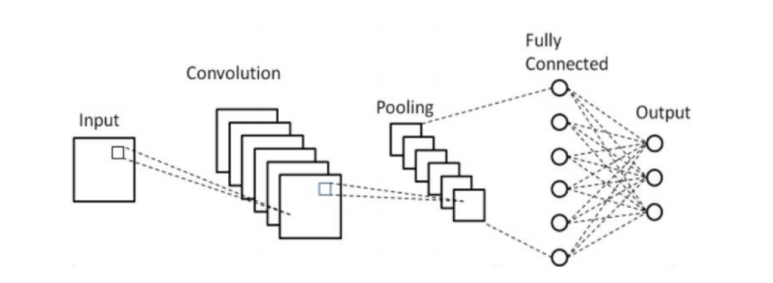
\includegraphics[width=0.7\textwidth]{img/cnn.png}
  \caption{Generalised Block Diagram of a CNN Model}
  \label{fig:cnn}
\end{figure}

\subsubsection{Recurrent Neural Networks and Long Short-Term Memory}

Recurrent Neural Networks (RNNs) extend feed-forward networks to handle
sequential data by maintaining a hidden state $h_t$ that is updated at each
time step $t$:

\begin{equation}
  h_t = \sigma\!\left(W_h\, h_{t-1} + W_x\, x_t + b\right)
\end{equation}

Plain RNNs suffer from vanishing and exploding gradients when sequences are
long. Long Short-Term Memory (LSTM) networks address this by introducing
gated memory cells. The update equations are:

\begin{align}
  f_t &= \sigma\!\left(W_f [h_{t-1}, x_t] + b_f\right) \\
  i_t &= \sigma\!\left(W_i [h_{t-1}, x_t] + b_i\right) \\
  \tilde{c}_t &= \tanh\!\left(W_c [h_{t-1}, x_t] + b_c\right) \\
  c_t &= f_t \odot c_{t-1} + i_t \odot \tilde{c}_t \\
  o_t &= \sigma\!\left(W_o [h_{t-1}, x_t] + b_o\right) \\
  h_t &= o_t \odot \tanh(c_t)
\end{align}
\noindent where $f_t$, $i_t$, $c_t$, and $o_t$ denote the forget gate, input gate,
cell state, and output gate respectively; $\odot$ denotes element-wise
multiplication. In handwriting recognition, LSTM networks are commonly
stacked bidirectionally (BiLSTM) so that each output position aggregates
context from both past and future time steps.

\subsubsection{Connectionist Temporal Classification (CTC)}

When a CNN-LSTM encoder produces a sequence of frame-level feature
vectors and the corresponding label sequence is shorter (as is typical for word
images), alignment between input frames and output characters is unknown
during training. CTC resolves this by marginalising over all possible
alignments. Given input length $T$ and target sequence $\mathbf{y}$ of length
$L$, CTC introduces a blank token $\varnothing$ and defines the loss as the
negative log-likelihood summed over all valid alignments $\pi$:

\begin{equation}
  \mathcal{L}_{\text{CTC}} = -\ln \sum_{\pi \,:\, \mathcal{B}(\pi) = \mathbf{y}}
  \prod_{t=1}^{T} p\!\left(\pi_t \mid \mathbf{x}\right)
\end{equation}
\noindent where the collapsing function $\mathcal{B}$ removes repeated characters and
blanks. CTC enables end-to-end training of sequence-to-label models without
requiring frame-level annotations.

\subsubsection{Transformer Architecture}

The Transformer is built entirely on
self-attention and dispenses with recurrence. Given an input sequence of
vectors $\mathbf{Z} \in \mathbb{R}^{n \times d}$, the scaled dot-product
attention is:

\begin{equation}
  \text{Attention}(Q, K, V)
  = \text{softmax}\!\left(\frac{QK^\top}{\sqrt{d_k}}\right)V
\end{equation}

\noindent where $Q$, $K$, and $V$ are linear projections of $\mathbf{Z}$.
Multi-Head Attention (MHA) runs $h$ independent attention heads in parallel and
concatenates their outputs:

\begin{equation}
  \text{MHA}(Q,K,V) = \text{Concat}(\text{head}_1, \ldots, \text{head}_h)\,W^O
\end{equation}

\noindent Each Transformer block couples MHA with a position-wise feed-forward network
(FFN) and applies layer normalisation with residual connections, enabling
gradient flow through very deep networks.

\subsubsection{Vision Transformer (ViT)}

The Vision Transformer (ViT) adapts the
Transformer encoder to image inputs by treating the image as a sequence of
non-overlapping patches. An image of size $H \times W$ is divided into
$N = HW / P^2$ patches of size $P \times P$ pixels. Each patch is flattened
and linearly projected to a $d$-dimensional embedding:

\begin{equation}
  \mathbf{z}_0 = [\mathbf{x}_{\text{cls}};\,
                  \mathbf{x}^1_p E;\; \mathbf{x}^2_p E;\; \ldots;\;
                  \mathbf{x}^N_p E] + \mathbf{E}_{\text{pos}}
\end{equation}

\noindent where $E \in \mathbb{R}^{(P^2 \cdot C) \times d}$ is the patch embedding
matrix and $\mathbf{E}_{\text{pos}}$ is a learnable positional encoding.
The sequence $\mathbf{z}_0$ is then processed by $L$ standard Transformer
encoder layers. Self-attention across patch tokens allows the model to capture
both local stroke features and long-range spatial relationships, which is
particularly beneficial for recognising structurally complex scripts like
Devanagari/Nepali.

\subsection{TrOCR: Transformer-Based OCR}

TrOCR \cite{li2023trocr} is an end-to-end transformer-based OCR model
that frames text recognition as an image-to-sequence problem. It follows
a standard encoder-decoder architecture in which the encoder extracts
visual features from the input image and the decoder autoregressively
generates the corresponding text sequence.

\begin{figure}[H]
  \centering
  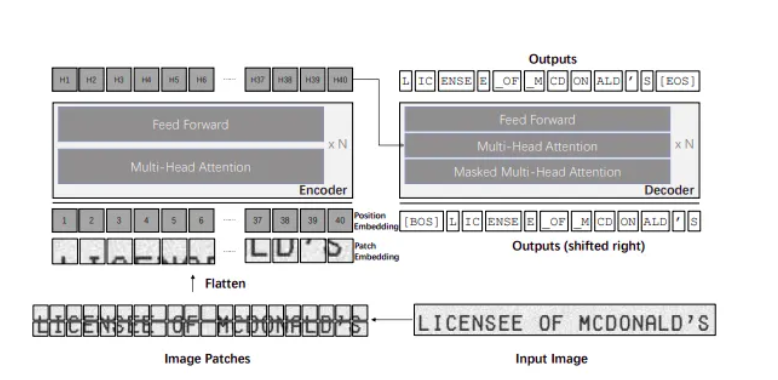
\includegraphics[width=0.80\textwidth]{img/theory.png}
  \caption{TrOCR Architecture}
  \label{fig:trocr}
\end{figure}

\subsubsection{Encoder}
The encoder is a Vision Transformer (ViT) that processes the input
image by first dividing it into a fixed grid of non-overlapping patches.
Each patch is linearly projected into a dense embedding vector, and
learnable position embeddings are added to retain spatial information.
The resulting sequence of patch embeddings is passed through a stack of
Transformer encoder layers, each comprising multi-head self-attention
and a position-wise feed-forward network. The output is a sequence of
contextual hidden states that collectively represent the visual content
of the image.

\subsubsection{Decoder}
The decoder is an autoregressive Transformer that generates the output
text one token at a time. It is initialised with a beginning-of-sequence
token \texttt{[BOS]} and continues generating tokens until the
end-of-sequence token \texttt{[EOS]} is produced. Each decoder layer
consists of three components: masked multi-head self-attention over
previously generated tokens, multi-head cross-attention over the encoder
hidden states, and a position-wise feed-forward network. At each
decoding step $t$, the model computes a probability distribution over
the vocabulary conditioned on all previously generated tokens and the
encoder output $\mathbf{H}$:
\begin{equation}
  p(y_t \mid y_{<t},\, \mathbf{H})
  = \text{softmax}\!\left(W_o\,
    \text{TransformerDecoder}(y_{<t},\, \mathbf{H})\right)
\end{equation}
The model is trained by minimising the cross-entropy loss over the full
target sequence:
\begin{equation}
  \mathcal{L} = -\sum_{t=1}^{T} \log p\!\left(y_t \mid y_{<t},\,
  \mathbf{H}\right)
\end{equation}
Both the encoder and decoder are initialised from large pre-trained
models, allowing TrOCR to leverage rich visual and linguistic
representations prior to task-specific fine-tuning.


\subsection{Dataset: IIIT-HW-Dev}

The IIIT Handwritten Devanagari (IIIT-HW-Dev) dataset
provides segmented word images of handwritten Devanagari script along with their Unicode ground-truth transcriptions. The dataset contains samples from multiple writers, covering a diverse vocabulary of Hindi/Nepali words. Eachimage has been pre-segmented at the word level, making it suitable for
word-image-to-text recognition without requiring additional line or word segmentation. The dataset is split into standard training, validation, and test partitions used throughout this work.

\subsubsection{Challenges of Devanagari Handwriting}

Devanagari/Nepali script presents several unique challenges for OCR:

\begin{itemize}
  \item \textbf{Conjunct consonants (half-characters):} Two or more consonants may combine into a single ligature, visually distinct from the base characters.
  \item \textbf{Matras (vowel diacritics):} Vowel signs attach above,below, or beside the base consonant, changing the visual appearance of the character significantly.
  \item \textbf{Headline (Shirorekha):} Most characters share a
horizontal headline stroke, causing characters within a word to be visually connected, complicating segmentation-based methods.
  \item \textbf{Inter-writer variability:} Stroke width, slant, and
    character proportions vary greatly across writers.
\end{itemize}

\noindent The end-to-end encoder-decoder approach adopted in this project directly
addresses these challenges by operating at the word-image level and relying on
the attention mechanism to learn character boundaries implicitly, without any
explicit segmentation step.

\newpage
\section{Review Matrix}



\setlength{\LTpre}{0pt}
\setlength{\LTpost}{0pt}
\renewcommand{\arraystretch}{1.3}
\noindent Table~\ref{tab:review-matrix} presents a summary of the literature reviewed in this chapter. It consolidates key studies, their methodologies, and contributions, providing a clear overview of the evolution of handwritten text recognition techniques.


\begin{longtable}[l]{|c|p{4.2cm}|c|p{3.5cm}|p{5cm}|}
\caption{Summary of Literature Review of NHWDTM system}
\label{tab:review-matrix} \\
\hline
\textbf{S.N.} &
\textbf{Title} &
\textbf{Year} &
\textbf{Algorithm} &
\textbf{Comments} \\ \hline
\endfirsthead

\multicolumn{5}{c}%
{\textbf{Table \thetable\ (continued)}} \\ \hline
\textbf{S.N.} &
\textbf{Title} &
\textbf{Year} &
\textbf{Algorithm} &
\textbf{Comments} \\ \hline
\endhead

% \hline \multicolumn{5}{r}{\textit{Continued on next page}} \\ \hline
\endfoot
\hline
\endlastfoot

1 & Handwritten Nepali character recognition and narration system \cite{baral2019handwritten} & 2019 & CNN & Built a foundational model to identify isolated Nepali characters, bypassing manual feature extraction. \\ \hline

2 & Evaluating sequence-to-sequence models for handwritten text recognition \cite{michael2019evaluating} & 2019 & Seq2Seq Models & Proved that sequence modeling is absolutely critical for mapping unsegmented image data directly to text. \\ \hline

3 & Nepali handwriting recognition using convolution neural network \cite{ghimire2020nepali} & 2020 & CNN, ANN & Optimized preprocessing stages to better handle the structural quirks of Devanagari scripts. \\ \hline

4 & An image is worth 16x16 words: Transformers for image recognition at scale \cite{dosovitskiy2020image} & 2020 & Vision Transformer (ViT) & Introduced ViT, proving self-attention on image patches could outperform traditional convolutions. \\ \hline

5 & iiit-indic-hw-words: A Dataset for Indic Handwritten Text Recognition \cite{10.1007/978-3-030-86337-1_30} & 2021 & Dataset Creation & Cleared a major data hurdle by providing a much-needed benchmark for Devanagari word-level OCR. \\ \hline

6 & Nepali handwritten character recognition system \cite{acharya2022nepali} & 2022 & CNN & Successfully utilized CNNs to convert handwritten Nepali text into an editable digital format. \\ \hline

7 & TrOCR: Transformer-based optical character recognition with pre-trained models \cite{li2023trocr} & 2023 & TrOCR (ViT + RoBERTa) & Introduced a brilliant end-to-end architecture that stripped away complex CNN backbones and CTC loss functions. \\ \hline

8 & Optical text recognition in Nepali and Bengali: A transformer-based approach \cite{hasan2023optical} & 2023 & Transformers & Achieved a massive leap in accuracy (WER of 0.15) for low-resource Indic scripts compared to traditional methods. \\ \hline

9 & Fine-tuning vision encoder-decoder transformers for historical documents \cite{parres2023fine} & 2023 & Vision Encoder-Decoder & Demonstrated the adaptability of vision encoder-decoder models on highly complex, cursive historical handwriting. \\ \hline

10 & Text detection and style classification from images Using ViT and transformer decoder \cite{yajima2024text} & 2024 & ViT, Transformer Decoder & Utilized Vision Transformers effectively to detect text and classify varied writing styles. \\ \hline

11 & HTR-VT: Handwritten text recognition with vision transformer \cite{li2025htr} & 2025 & ViT, SAM & Hit state-of-the-art results by combining Vision Transformers with sharpness-aware minimization. \\ \hline

12 & Automated Handwriting Pattern Recognition for mutlti-level personality classification using transformer ocr \dots Using TrOCR \cite{inproceedings} & 2025 & TrOCR & Showcased TrOCR's incredible adaptability for complex automated handwriting pattern classification tasks. \\ \hline

13 & Transforming images into words: optical character recognition solutions for image text extraction \cite{article} & 2025 & Comprehensive Review & Reinforced that Transformer architectures are the undeniable new gold standard for image text extraction. \\ \hline

14 & Enhancing Accuracy in Indic Handwritten Text Recognition \cite{10.1007/978-3-031-93688-3_17} & 2026 & Deep Learning / HTR & Explored crucial new techniques to handle cursive Devanagari, reinforcing the need for sequence-aware architectures. \\ \hline
\end{longtable}


    \chapter{METHODOLOGY}
\label{ch:methodology}

This chapter describes how the system was built, in the order the work was carried out. The pipeline runs from establishing the signed form of each phrase with Deaf experts, through recording and preprocessing a custom dataset, to training the classifier, evaluating it, and deploying it. The evaluation protocol and the deployment path are described at the end, since both differ from what the proposal anticipated.

\section{Software Development Approach}

Agile incremental development was adopted because several parameters could not be fixed in advance. The sequence length depended on how long signers actually took to perform each phrase, the normalisation scheme had to be validated against real recordings, and the deployment target changed once the recognition results were in hand. Each increment delivered a working module: phrase verification, the recorder, the preprocessing core, the trained model, the inference server, and the mobile client.

The riskiest unknown was addressed first. Before any large-scale recording, a small set of clips was captured to confirm that MediaPipe Holistic produces stable landmarks for multi-sign NSL phrases performed at natural speed. Had it not, the entire landmark-based approach would have needed reconsideration while there was still time to change it.

\begin{figure}[H]
    \centering
    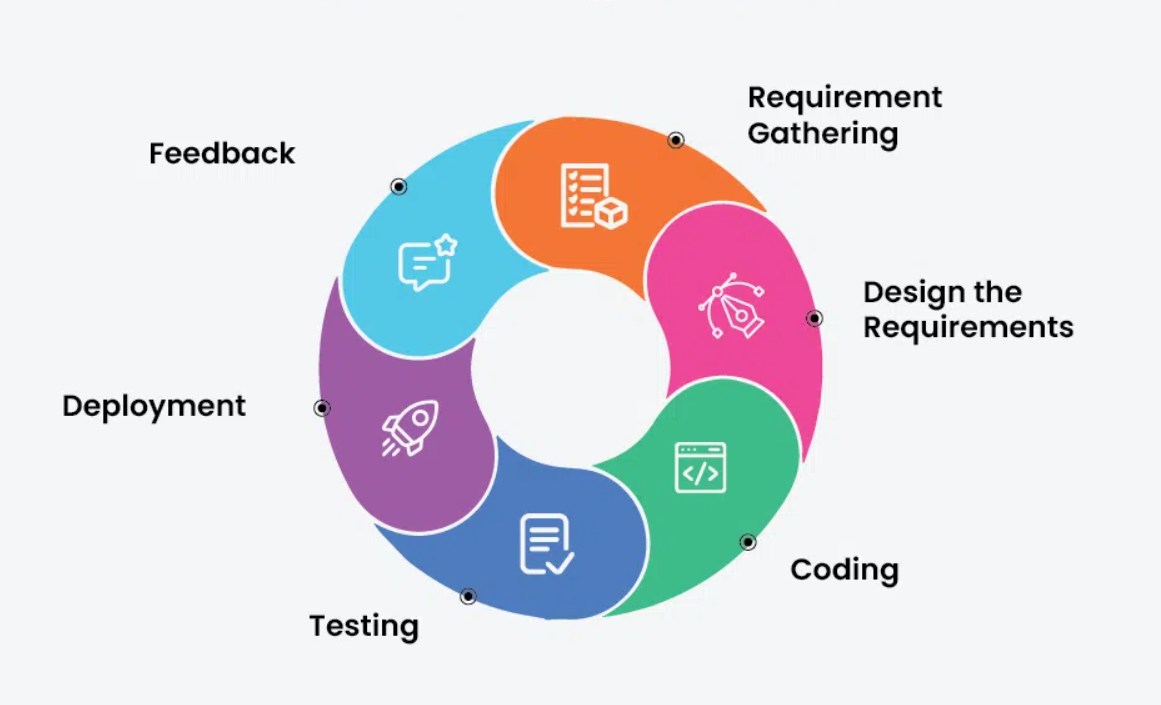
\includegraphics[width=0.7\textwidth]{img/sdlc.png}
    \caption{Agile incremental development approach}
    \label{fig:agile}
\end{figure}

\section{Phase 0: Establishing the Signed Form of Each Phrase}
\label{sec:phase0}

No standard published gloss exists for the six target emergency phrases, so the natural signed form of each had to be established with the Deaf community before recording could begin. Two consultations were held in person: with Yojana Sakha and colleagues at the Rehabilitation Centre for the Rural Deaf in Bhaktapur, and with a resource person at the National Federation of the Deaf Nepal in Ranibari Marga, Samakhushi, Kathmandu.

Each consultant was asked to demonstrate how the idea would be signed in an actual emergency, as concisely as possible, and not to sign the English sentence word by word. Each demonstration was discussed for regional variation, recorded as a reference, and confirmed as the form every signer would reproduce. Because the experts' time was limited, they also contributed roughly ten clips per phrase, which anchor the dataset to an authentic performance. Photographs from the consultations appear in Appendix~\ref{app:fieldwork}.

The consultants were also asked directly whether facial expression changes or adds meaning for any of the six phrases. They confirmed it does not for this phrase set, which settled the exclusion of the 468 face landmarks from the feature vector.

Table~\ref{tab:phrases} lists the six phrases and the situation each covers. Phrase 6 replaced an earthquake phrase considered at proposal stage. The consultants advised that a request to use the toilet is a far more frequent communication failure for deaf people in institutional settings than an earthquake report, and the change was approved at the mid-term defence.

\begin{table}[H]
    \centering
    \caption{Target emergency phrases and their categories}
    \label{tab:phrases}
    \small
    \begin{tabular}{|c|p{3.6cm}|p{3.4cm}|l|l|}
        \hline
        \textbf{\#} & \textbf{English phrase} & \textbf{Nepali phrase} & \textbf{Category} & \textbf{Class key} \\
        \hline
        1 & I can't breathe            & \nepali{मलाई सास फेर्न गाह्रो भइरहेको छ} & Medical           & \texttt{cant\_breathe} \\
        \hline
        2 & The building is on fire    & \nepali{भवनमा आगो लागेको छ} & Fire              & \texttt{building\_on\_fire} \\
        \hline
        3 & Call the police            & \nepali{प्रहरीलाई फोन गर्नुहोस्} & Crime             & \texttt{call\_police} \\
        \hline
        4 & I need an ambulance        & \nepali{मलाई एम्बुलेन्स चाहियो} & Medical           & \texttt{need\_ambulance} \\
        \hline
        5 & Help me / I am in danger   & \nepali{मलाई मद्दत गर्नुहोस् / म खतरामा छु} & Generic emergency & \texttt{help\_danger} \\
        \hline
        6 & I need to go to the toilet & \nepali{मलाई शौचालय जानु छ} & Basic need        & \texttt{need\_toilet} \\
        \hline
        7 & Not one of the above       & --- & Negative class    & \texttt{none} \\
        \hline
    \end{tabular}
\end{table}

\subsection{The Negative Class}

The seventh class was added during development and is not in the original proposal. A classifier over six phrases assigns one of those six to every input it receives, so a signer adjusting their glasses would be reported as an emergency. For a system whose output is a spoken emergency announcement, that is the worst available failure mode.

The \texttt{none} class holds deliberate non-examples: resting, idle movement, gestures outside the target set, and partial or abandoned signs. Giving the model explicit negatives lets it learn a decision boundary around the six real phrases instead of partitioning the whole input space among them, so the confidence threshold of Section~\ref{sec:decisionrule} has a class to fall back on instead of being forced to choose one of six emergency phrases for every input.

\section{Phase 1: Dataset Collection}

Because no public dataset of NSL emergency phrases exists, one was recorded from scratch. This was the most consequential phase of the project: the ceiling on recognition accuracy is set by the quality and variety of the recordings.

\subsection{The Recorder Application}

A purpose-built recorder was written for the task. It runs MediaPipe Holistic live on a webcam feed and, for every frame, extracts a 225-value vector: 33 pose landmarks, 21 left-hand landmarks, and 21 right-hand landmarks, each with $x$, $y$, and $z$ coordinates. The operator selects a signer identity and a phrase, then starts and stops each recording explicitly, so every clip corresponds to one deliberate performance of one phrase.

Every frame is mirrored horizontally before detection. This is recorded here because it is a constraint on everything downstream: the landmarks in the dataset describe a mirrored image, and any inference path that does not reproduce the same flip will present the model with the signer's hands swapped. Screenshots of the recorder in use appear in Appendix~\ref{app:recorder}.

Frames in which a hand or the pose is not detected are zero-filled for that block and the detection rate is recorded. The frame is not dropped. Each clip is therefore accompanied by a JSON sidecar holding its frame count, duration, and per-block detection rates, which made it possible to identify weak recordings without replaying them.

\subsection{Recording Setup and Variation}

Variation was introduced deliberately so the model would not learn a single recording condition:

\begin{itemize}
    \item Lighting: bright, dim, and mixed daylight near a window.
    \item Background: plain wall, cluttered room, and several different rooms.
    \item Distance: close to the camera and at arm's length or further.
    \item Signers: eight people, differing in body size, hand size, and signing speed.
    \item Speed: each signer performed each phrase somewhat faster and somewhat slower across takes.
\end{itemize}

Each clip is saved as \texttt{<phrase>\_\_<signer>\_\_<index>.npy}. Encoding the signer in the filename is what makes signer-independent evaluation possible later, and it was the reason for adopting the convention.

\subsection{Storing Landmarks Instead of Video}

The recorder saves only the per-frame landmark vectors. Video is never written to disk. This keeps the dataset small, removes a slow reprocessing step from every later stage, and means no video of any signer is stored or transmitted.

The cost is worth stating plainly. Because no video was kept, the landmark representation cannot be recomputed. Changing the landmark source, for example to run detection on a phone instead of a server, cannot be evaluated against the existing data and would require re-recording every clip.

\subsection{Aggregation Across Signers}

The eight signers recorded independently on separate machines. Git was used to merge each contribution into one shared repository instead of copying files by hand, which gave a reviewable history of what each signer added and caught duplicate and misnamed clips before they entered the combined set. Screenshots of the merged repository and the resulting directory layout appear in Appendix~\ref{app:dataorg}.

After aggregation the dataset held 840 clips: exactly 120 in each of the seven classes, contributed by eight signers. The composition is reported in full in Section~\ref{sec:datasetcomposition}.

\section{Phase 2: Feature Extraction}

Every frame of every clip is reduced to the same 225-dimensional vector, concatenated in a fixed order:

\begin{itemize}
    \item 33 pose landmarks $\times\ (x, y, z)$ = 99 values, at indices 0 to 98.
    \item 21 left-hand landmarks $\times\ (x, y, z)$ = 63 values, at indices 99 to 161.
    \item 21 right-hand landmarks $\times\ (x, y, z)$ = 63 values, at indices 162 to 224.
\end{itemize}

\noindent A clip is therefore a $(n_{\text{frames}}, 225)$ array of 32-bit floats, with $n_{\text{frames}}$ varying between clips. This layout, the normalisation anchors, and the sequence length are held as constants in a single module that both the training code and the inference server import, so the two cannot drift apart.

\section{Phase 3: Determining the Sequence Length}

The classifier requires a fixed number of time steps, but raw clip lengths vary because signers take different amounts of time. The value was measured from the data rather than chosen.

Across the 840 clips, frame counts ranged from 18 to 217, with a median of 89 and a mean of 90.1. The 95th percentile of this distribution gives $\textsc{seq\_len} = 137$ frames. The distribution and the cutoff are shown in Figure~\ref{fig:seqlen} in Chapter~\ref{ch:results}. The value is written to a metadata file that every later stage reads, so no stage recomputes or assumes it.

An observation from the same metadata turned out to matter more than expected. The recorder never locked a frame rate; it ran as fast as the interface and MediaPipe allowed, giving a median capture rate of 15.7 frames per second across a range of 10.8 to 21.2. Since the model receives a fixed-length sequence with no explicit time axis, it reads frame count as duration. The capture rate is therefore a property of the training data that any real-time path has to reproduce, and Section~\ref{sec:framerate} describes how.

\section{Phase 4: Normalisation and Standardisation}

Each clip is normalised and then standardised to \textsc{seq\_len}, in that order.

Normalisation applies the dual-anchor scheme of Section~\ref{sec:normalisation} to each frame, treating the three landmark blocks independently. The pose block is re-centred on the shoulder midpoint and divided by shoulder width; each hand block is re-centred on its wrist and divided by the wrist-to-middle-knuckle distance. Normalising per block keeps the position of a hand relative to the body while removing the signer's position and distance from the camera.

Standardisation then forces the clip to exactly 137 frames in one of three ways. A clip already at 137 frames is used unchanged. A longer clip is subsampled at 137 evenly spaced positions spanning its full duration, so the whole performance is represented instead of the first 137 frames. A shorter clip is zero-padded at the end, and a boolean mask records which frames are real.

The order is what makes the padding safe. Both normalisation formulas map a zero input to zero output, so an undetected block stays zero through normalisation, and padding added afterwards is also exactly zero. The classifier's masking layer then skips any all-zero time step at no cost. Padding after normalising would have produced non-zero padded frames that the model would read as signal.

The compiled dataset is stored as three aligned arrays: the normalised sequences with shape $(840, 137, 225)$, the integer labels with shape $(840,)$, and the padding mask with shape $(840, 137)$. A manifest records the class, signer, source file, and original frame count for every row, which keeps each compiled clip traceable to the recording it came from.

\section{Phase 5: Model Training}

\subsection{Architecture}

The classifier is a bidirectional LSTM built with TensorFlow and Keras:

\begin{table}[H]
    \centering
    \caption{Classifier architecture}
    \label{tab:architecture}
    \begin{tabular}{|l|l|}
        \hline
        \textbf{Layer} & \textbf{Purpose} \\
        \hline
        Input $(137, 225)$              & one normalised clip \\
        \hline
        Masking (mask value 0.0)        & skips zero-padded and undetected frames \\
        \hline
        Bidirectional LSTM, 64 units    & reads the motion in both directions \\
        \hline
        Dropout 0.3                     & regularisation \cite{srivastava2014dropout} \\
        \hline
        Bidirectional LSTM, 32 units    & summarises the sequence \\
        \hline
        Dropout 0.3                     & regularisation \\
        \hline
        Dense 32, ReLU                  & feature layer feeding the classification head \\
        \hline
        Dense 7, softmax                & probability over the seven classes \\
        \hline
    \end{tabular}
\end{table}

\noindent The network has 192{,}007 trainable parameters, which is small enough to train on a laptop CPU in minutes.

\subsection{Why This Model and Not a Larger Pretrained One}

A dataset of 840 clips is small for a network trained from scratch, which raises the
question of whether a pretrained model should carry more of the work. The answer is that
one already does, and that the division of labour is where the data efficiency comes from.

MediaPipe Holistic is the pretrained component. It was trained on far more human pose and
hand data than this project could ever collect, and it performs the part of the task that
needs that scale: locating a body and two hands in an arbitrary image under arbitrary
lighting. What reaches the BiLSTM is not an image but 225 already-interpreted coordinates,
so the only thing left to learn is how those coordinates move over time for each phrase.
That is a much smaller problem, and 192{,}007 parameters is a proportionate model for it.

A pretrained video classifier operating on pixels was considered and rejected for two
reasons. It would need the raw video, which was deliberately never stored, so adopting one
would mean re-recording the entire dataset. It would also be too large for the deployment
target, where the whole exported model is 879 kilobytes and runs without a GPU.

The dataset was also enlarged during development in preference to adding model capacity,
growing from four signers and 570 clips at the mid-term to eight signers and 840 clips.
For a landmark-based classifier at this vocabulary size, additional signers buy more than
additional parameters, because the quantity in short supply is variation between people and
not model expressiveness.

\subsection{Training Configuration}

Training minimises sparse categorical cross-entropy with the Adam optimiser \cite{kingma2015adam} at a batch size of 16, for at most 200 epochs. Class weights are computed to be inversely proportional to class frequency, which matters more for the folds than for the whole dataset, since the classes are balanced overall but a held-out signer's contribution is not always uniform.

Two callbacks control the schedule. Early stopping monitors validation loss with a patience of 15 epochs and restores the best weights. Its minimum-improvement threshold is set to $10^{-3}$ and not left at zero, because with a threshold of zero any improvement at all resets the patience counter, including a change in the fourth decimal place. Once validation loss approaches zero it keeps setting negligible new records, so training does not end on convergence; it ends whenever an optimiser instability finally breaks the streak. That made the epoch count a record of when a random fluctuation occurred instead of a property of the fit.

Learning rate reduction on plateau addresses the cause of those fluctuations, halving the learning rate after 6 epochs without improvement, down to a floor of $10^{-5}$. Its patience is kept well below the early-stopping patience so that the reduced rate has a chance to take effect before training halts.

Reproducibility required more than fixing the random seed. TensorFlow's parallel CPU reductions vary between runs, and on identical data this moved per-fold accuracy by up to 2.7 percentage points. Deterministic operations are therefore enabled explicitly, at some cost in speed, so that a reported fold accuracy is a property of the data and the recipe, not of one particular run.

\section{Phase 6: Evaluation Methodology}

\subsection{Leave-One-Signer-Out}

The headline metric is leave-one-signer-out accuracy. For each signer eligible to be held out, the model is trained from scratch on every clip from the other signers and tested only on that signer's clips. Within each fold, 15\% of the training clips are set aside as a stratified validation split for early stopping, so the held-out signer influences neither the fitted weights nor the stopping point.

A signer is eligible for holdout only if removing their clips leaves every class present in the remainder. All eight signers satisfied this, giving eight folds. Two figures are reported: the mean accuracy across folds, which estimates performance on a new person, and the pooled accuracy over all 840 predictions, where each clip is scored exactly once by a model that never saw its signer.

\subsection{The Random-Split Contrast}

A stratified 70/15/15 random split is also trained and reported. It is not an additional performance measure. Its purpose is to quantify what the signer-independent protocol is protecting against: under a random split, clips from the same person appear in both training and test, and the model can score well by recognising individuals. The gap between the two protocols is the size of that effect on this dataset, and it is discussed in Section~\ref{sec:leakage}.

\subsection{Metrics}

Overall accuracy is reported alongside per-class precision, recall, and F1:
\begin{equation}
    \text{Precision} = \frac{TP}{TP+FP}, \quad
    \text{Recall} = \frac{TP}{TP+FN}, \quad
    \text{F1} = \frac{2\,\text{Precision}\cdot\text{Recall}}{\text{Precision}+\text{Recall}}.
\end{equation}
A confusion matrix pooled over all folds identifies which classes are mutually confusable. For an emergency system the two directions of error are not equivalent: failing to recognise a real phrase leaves the user without help, while announcing a phrase for a non-sign produces a false alarm. Both appear in the matrix and are discussed separately.

\section{Phase 7: Deployment}

\subsection{Revision of the Deployment Approach}
\label{sec:deploychange}

The proposal specified a browser application built with Next.js, running the model in the visitor's browser through TensorFlow.js, with no server involved. The delivered system is an Android application that streams frames to an inference server. Two separate decisions produced that change and they are worth separating.

The first is the choice of device. A phone is what a person has with them when an emergency happens; a laptop with a browser open is not. For a tool whose value depends on being available at the moment of need, the phone is the correct target, and this was decided on those grounds. The browser route was not attempted. The change was recorded as a task deviation in the project log and accepted by the supervisor before the client was built.

The second decision concerns where inference runs, and it carries a real cost. MediaPipe Holistic, the exact landmark extractor the dataset was recorded with, exists as a Python pipeline. Running recognition on the device would mean reimplementing the 225-feature extraction and the dual-anchor normalisation against a different landmark source, and a numerical difference between the two implementations does not raise an error. It produces confident wrong answers, because the model receives numbers unlike anything it was trained on. Serving from Python means the inference path imports the same preprocessing module that the reported accuracy was measured with, so the correspondence between measured and deployed behaviour is structural, not something that had to be verified.

The cost is that the delivered system requires a network connection at use time, which the proposal stated it would not. For an emergency tool this is a genuine weakness and not a neutral trade. It is listed among the limitations in Chapter~\ref{ch:conclusion}, along with the work that would remove it.

\subsection{Model Export}

The trained model is converted to TensorFlow Lite \cite{tflite2024} so the server can run it without a full TensorFlow installation, reducing the deployed image from about three gigabytes to one. The conversion required a workaround: on the pinned TensorFlow and Keras versions used here, the standard converter entry points abort the host process inside the compiler backend instead of raising a catchable exception. Freezing the model's variables to constants before conversion avoids the failure.

Because a silent conversion error would be indistinguishable from a model that simply performs worse, the export is verified and not assumed. The converted model and the original are run on 30 real clips and compared; the export is rejected if they disagree. The measured agreement is reported in Section~\ref{sec:exportverify}.

\subsection{Inference Server}

The server is a FastAPI application exposing a WebSocket endpoint. A client opens a session, streams JPEG frames while the user signs, and sends a completion message; the server replies with the decision. Landmark extraction costs about 38 milliseconds per frame and accounts for almost the entire pipeline cost, so streaming frames during signing overlaps that work with the signing itself. When the client signals completion, only normalisation, standardisation, and the forward pass remain, which together take about 15 milliseconds. Uploading a finished recording instead would have serialised the two and added several seconds of silence before every result.

Each session holds its own MediaPipe graph, which occupies about 150 megabytes, so concurrency is bounded by memory, not processor time. A semaphore caps simultaneous sessions and refuses further connections with an explicit error instead of allowing the process to be killed for exhausting memory. Requests are authenticated with a shared key compared using a constant-time function, so that a wrong key cannot be narrowed down by timing the response. The health endpoint is left unauthenticated so that container health checks and the client's reachability test continue to work.

\subsection{Frame Rate as a Correctness Constraint}
\label{sec:framerate}

Because the model reads frame count as duration, a client capturing at 30 frames per second produces twice as many frames for the same sign as the training data contained, and presents the model with a temporal scale it has never seen. The server therefore discards incoming frames down to the 15.7 frames per second of the training data before running detection, using an accumulator that tracks when the next frame is due. A simpler test of whether enough time has elapsed since the last accepted frame aliases a 16 frames-per-second client down to 8. The client caps its own send rate at 16 frames per second, slightly above the target so that jitter does not starve the server below it.

\subsection{Mobile Client}

The Android client performs no recognition. It captures camera frames, encodes them, sends them, and speaks the result.

Frame encoding is the client's bottleneck, since it is pure Dart. Colour conversion, rotation, and downscaling are folded into a single pass over the output pixels, avoiding the intermediate full-resolution buffers a naive implementation allocates. Frames are downscaled to 320 pixels wide and encoded with chroma subsampling, on the grounds that landmarks are derived from luminance structure and not chroma resolution. The work runs on a persistent background isolate. When a frame is already in flight the next one is dropped instead of queued, since the server discards surplus frames anyway and a queue would only add latency.

Two details are recorded because they are easy to get wrong. The application is locked to portrait orientation and rotates each frame by the camera's sensor orientation before sending, because Android delivers frames in sensor orientation and MediaPipe detects nothing at all in an image of a person lying sideways. Frames are sent unmirrored with a flag instructing the server to apply the same horizontal flip the recorder used, and the flag is set for both front and rear cameras: the lens faces the signer either way, so the signer's right hand appears on the image-left in both cases, and making the flag depend on the camera would swap the two hand blocks in the feature vector for one of them.

\subsection{The Decision Rule}
\label{sec:decisionrule}

Two outcomes are possible:

\begin{enumerate}
    \item If the predicted class is one of the six emergency phrases and the softmax confidence reaches 0.75, the result is \texttt{accepted}. The phrase is displayed and spoken.
    \item Otherwise the result is \texttt{low\_confidence}. This covers a prediction of the \texttt{none} class and a low-confidence prediction of any class alike: the user is told the input was not recognised clearly, and nothing is spoken.
\end{enumerate}

\noindent Folding rejection into the classifier this way keeps a wrong announcement and no announcement on the same footing: both routes into \texttt{low\_confidence} withhold output rather than guessing. The best guess and the top three probabilities are returned in every case, including refusals, which is what makes a failure diagnosable during a demonstration.

    \chapter{SYSTEM DESIGN}

\section{Requirement Specification}

\subsection{Functional Requirements}
\begin{itemize}
    \item \textbf{Input Handling:} The system accepts handwritten Nepali word images from the IIIT-HW-Dev dataset during training and evaluation, as well as user-provided images during inference.

    \item \textbf{Image Pre-processing:} Input images are automatically passed through a multi-step pipeline comprising grayscale conversion, denoising, adaptive binarisation, morphological closing, deskewing, tight cropping, and letterbox padding to $128 \times 128$ pixels, followed by rescaling to $384 \times 384$ pixels and normalisation by the ViTImageProcessor to match the ViT encoder's pre-training distribution.

    \item \textbf{Feature Extraction and Recognition:} The pre-trained ViT encoder extracts a contextual visual feature matrix from the input image, and the custom BERT-based decoder  attends to these features via cross-attention to autoregressively generate the corresponding Nepali Unicode word.

    \item \textbf{Tokenization:} A custom character-level tokenizer encodes ground-truth Unicode labels into integer token sequences and decodes predicted token IDs back into Devanagari text using a 112-token vocabulary.

    \item \textbf{Training and Evaluation:} The system is trained using label-smoothed cross-entropy loss and evaluated using Character Error Rate (CER), Word Error Rate (WER), Exact Match Accuracy, and Normalised Edit Distance (NED).

    \item \textbf{Inference:} The model generates predictions using beam search decoding (num\_beams = 4)), returning the top 3 candidate transcriptions ranked by sequence log-probability score.

    \item \textbf{Output:} The primary output is the highest-scoring candidate Nepali word in Unicode format. For single-image inference, two additional confidence signals are reported:
\begin{enumerate}
    \item Per-character confidence, expressed as a percentage derived from 
    per-token transition probabilities.
    \item Sequence-level beam scores (log-probability) for each of the top 
    3 alternative predictions, allowing the user to assess and manually 
    select a more appropriate candidate if needed.
\end{enumerate}
\end{itemize}

\subsection{Non-Functional Requirement}
\begin{itemize}
    \item \textbf{Performance:} The system should provide accurate predictions with reasonable response time using GPU acceleration.

    \item \textbf{Scalability:} The model can be extended to process full sentences or paragraphs by adding a word segmentation module.

    \item \textbf{Accuracy:} The system aims to achieve low CER and WER, and high Exact Match Accuracy on the test dataset.

    \item \textbf{Usability:} The model should be easy to use and deploy as a standalone tool or API for digitizing handwritten documents.

    \item \textbf{Reliability:} The system should produce consistent results across different handwriting styles.
\end{itemize}
\newpage
\section{Use Case Diagram}
      The Use Case Diagram \ref{fig:use case diagram} illustrates the interaction between the actor and the Nepali Handwritten Word Recognition System.
    \begin{figure}[H]
        \centering
        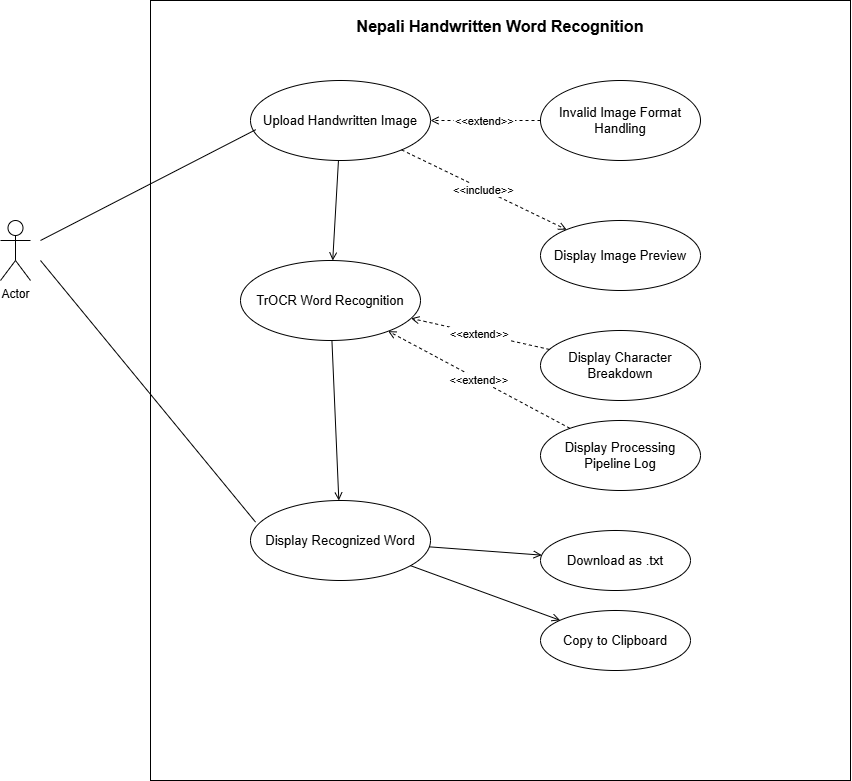
\includegraphics[scale=0.5]{img/UCD.png}
        \caption{Use Case Diagram of Nepali Handwritten Word Digitization}
        \label{fig:use case diagram}
   \end{figure}
     \noindent The process begins when the user uploads a handwritten image, which automatically includes displaying an image preview and may extend to handle invalid image formats. The uploaded image is directly passed into the TrOCR Word Recognition process, which may optionally extend to display a character breakdown. Finally, the recognized word is displayed to the user, with additional options to download the result as a .txt file or copy it to the clipboard.
%\section{Activity Diagram}
   % \begin{figure}[H]
      %  \centering
        %\includegraphics[scale=0.69]{img/ActivityDiagram.png}
       % \caption{Activity Diagram}
       % \label{fig:activity diagram}
  % \end{figure}
 %  The activity diagram illustrates the complete workflow of the system from start to finish. The process begins when the user uploads a handwritten image. If the image format is invalid, an error message is displayed and the process terminates. If the format is valid, the image preview is shown and the image enters the preprocessing pipeline, which consists of grayscale conversion, binarization, deskewing, and tight cropping. The preprocessed image is then fed into the fine-tuned TrOCR model to generate Unicode Nepali text. The post-processing stage runs in parallel to display the recognized word, generate a character-level confidence breakdown, and produce a pipeline processing log. Finally, if the user chooses to export the result, they can either download it as a .txt file or copy it to the clipboard, after which the process ends.

\newpage
\section{Class Diagram for System}
This class diagram \ref{fig:classdiagram} illustrates the structure of the Nepali Handwritten Word Recognition System.
\begin{figure}[H]
    \centering
    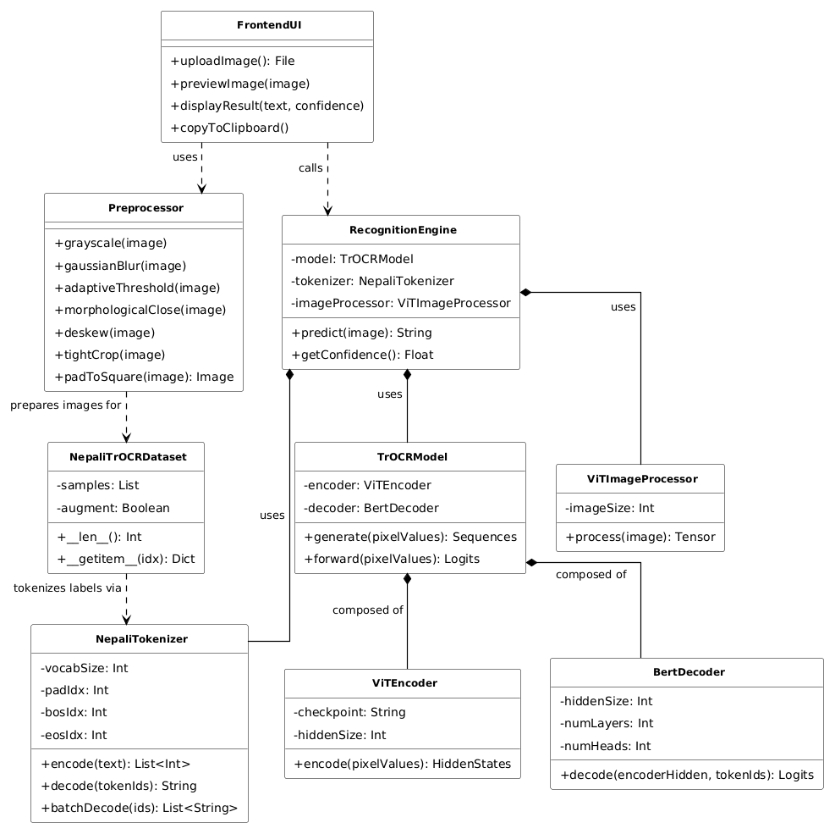
\includegraphics[width=\textwidth]{img/ClassDiagram.png}
    \caption{Class diagram of Nepali Handwritten Word Digitization}
    \label{fig:classdiagram}
\end{figure}
 \noindent The FrontendUI is the entry point where the user uploads a handwritten word image and receives the predicted text with confidence scores. It directly interacts with the Preprocessor, which cleans the image through a seven-step pipeline, and the RecognitionEngine, which handles inference. The preprocessed images feed into the NepaliTrOCRDataset, which uses the NepaliTokenizer to convert Devanagari labels into character-level token IDs. During inference, the RecognitionEngine coordinates the TrOCRModel, NepaliTokenizer, and ViTImageProcessor. The TrOCRModel is composed of a pretrained ViT encoder and a lightweight custom BERT-based decoder consisting of two layers, four attention heads, hidden size 256 to generate the recognised character sequence. Each class has a single well-defined responsibility, ensuring a clean data flow from raw handwritten input to Unicode text output.



  
%\section{Class Diagram for Data }

%\section{Database Schema}

\section{Sequence Diagram}
The sequence diagram \ref{fig:sequence diagram} depicts the step-by-step interaction between the system components during a recognition request. The user uploads a handwritten image through the Frontend UI, which previews the image before the user initiates recognition. The frontend sends a POST request to the FastAPI Backend, which forwards the image to the Preprocessor. The Preprocessor applies grayscale conversion, binarization, deskewing, and tight cropping before returning the cleaned image to the backend.
    \begin{figure}[H]
        \centering
        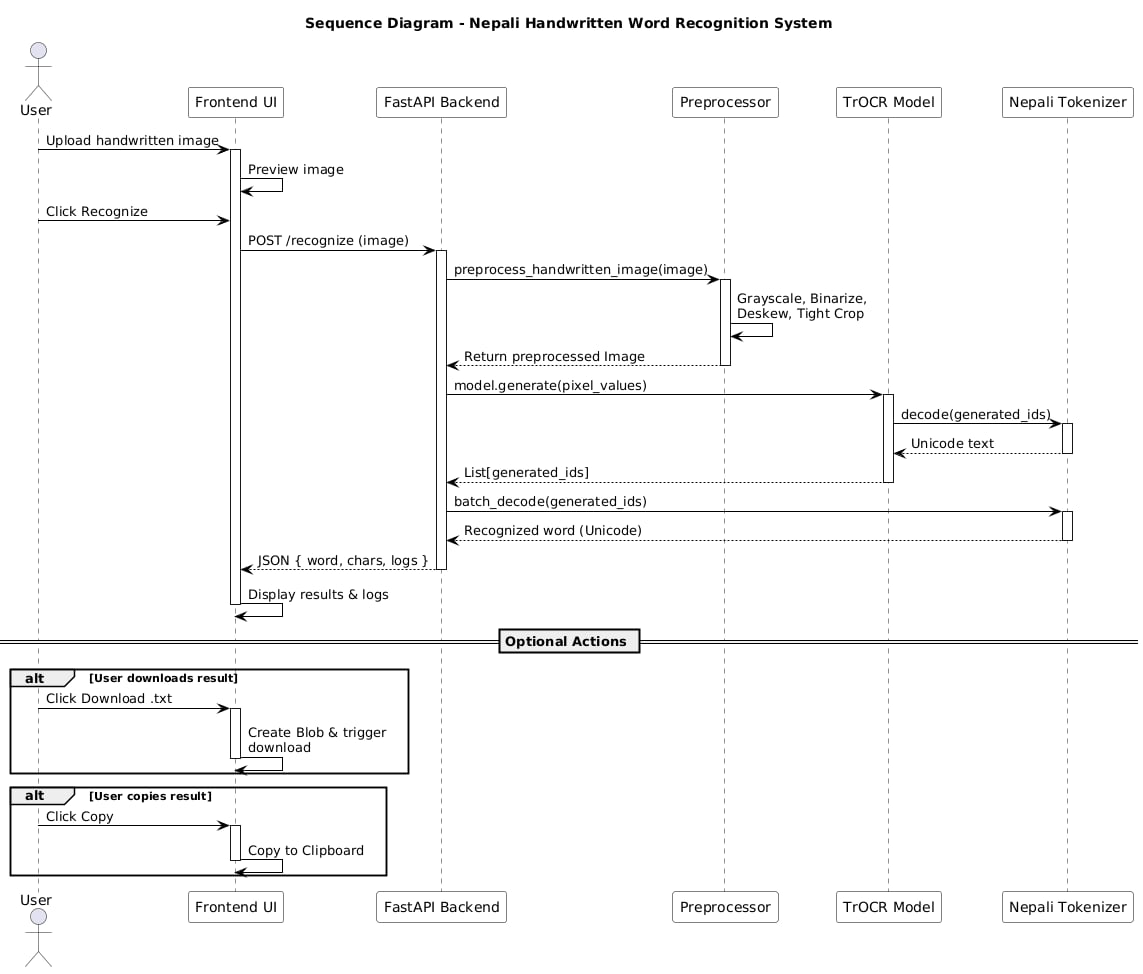
\includegraphics[scale=0.4]{img/SD.jpg}
        \caption{Sequence Diagram of Nepali Handwritten Word Digitization}
        \label{fig:sequence diagram}
   \end{figure}
   \noindent The backend then calls the TrOCR Model to generate token IDs, which are decoded into Unicode text by the Nepali Tokenizer. The final recognized word is returned to the frontend as a JSON response and displayed to the user. Optionally, the user may download the result as a .txt file or copy it to the clipboard.

%\section{Data Flow Diagram}

   % \begin{figure}[H]
      %  \centering
       % \includegraphics[scale=0.38]{img/dfd0.png}
       % \caption{Level 0 Data Flow Diagram}
       % \label{fig:Level 0 Data Flow Diagram}
  % \end{figure}
  % The context diagram provides a high-level overview of the system. The user provides a handwritten image as input to the Nepali Handwritten Word Recognition System. The system processes the image and returns the recognized Unicode Nepali text, downloadable output, and confidence logs back to the user. Any invalid image format triggers an error notification.

   % \begin{figure}[H]
      %  \centering
       % \includegraphics[scale=0.5]{img/Level1.jpg}
      %  \caption{Level 1 Data Flow Diagram}
       % \label{fig:Level 1 Data Flow Diagram}
   %\end{figure}
%\noindent
%The Level 1 Data Flow Diagram breaks down the internal processes of the system. The user submits a handwritten image which enters the Upload Image process. The raw image is then passed to the Preprocess Image process where it is cleaned and normalized. The cleaned image is fed into the Run TrOCR Inference process, which loads model weights from the TrOCR Model data store. The generated token IDs are passed to the Decode Output process, which references the Nepali Tokenizer data store to map tokens to Unicode characters. The resulting Unicode text is then passed to the Display Result process, which returns the recognized word and character breakdown to the user.





%\section{Deployment Diagram}
%\textbf{Note: All the diagram is not mandatory..select according to the type of project you are going to do.}
    \chapter{RESULT AND DISCUSSION}


\section{Experiment Setup}
All experiments were conducted on Kaggle's cloud-based GPU infrastructure.
Table~\ref{tab:hardware} summarises the hardware and software environment used
throughout training and evaluation.
 
\begin{table}[h!]
\centering
\renewcommand{\arraystretch}{1.1} 
%\large
\begin{tabular}{|l|l|}
\hline
\textbf{Component} & \textbf{Specification} \\ \hline
GPU                      & NVIDIA Tesla T4 (16 GB VRAM) \\ \hline
System RAM               & 29 GB \\ \hline
Operating System         & Linux (Ubuntu 20.04) \\ \hline
Python                   & 3.10 \\ \hline
PyTorch                  & 2.1 (CUDA 12.1) \\ \hline
HuggingFace Transformers & 4.40 \\ \hline
Training Precision       & fp16 (mixed precision) \\ \hline
Training Platform        & Kaggle Notebooks \\ \hline
\end{tabular}
\vspace{2pt} % Adds a small gap between table and caption
\caption{Hardware and software environment}
\label{tab:hardware}
\end{table}

\section{Training Configuration}

Four model configurations were explored during the course of this project,each differing in encoder backbone and decoder architecture.

\noindent The Baseline model retained the original RoBERTa-based decoder from microsoft/trocr-base-handwritten with the Devanagari character set
added to its existing vocabulary. While this required minimal changes, the RoBERTa decoder had been pre-trained on English text, causing it to treat
Devanagari characters as rare multi-byte fallback tokens and producing excessively long, fragmented token sequences with poor generation coherence for Nepali words.

\noindent The TrOCR-Small variant replaced the ViT-Base encoder with a ViT-Small encoder of approximately 22 million parameters. Although this reduced memory usage and training time, the smaller encoder capacity limited the richness of visual features available for structurally complex conjunct consonants and compound Devanagari characters, resulting in higher recognition errors on difficult word forms.

\noindent The TrOCR-Large variant used a ViT-Large encoder with 307 million parameters across 24 transformer layers, paired with a larger custom BERT
decoder of 4 layers and 8 attention heads. While the larger encoder provided richer visual representations, the substantially increased memory footprint made full Phase~2 fine-tuning impractical on the available Kaggle GPU infrastructure, restricting the number of training epochs and limiting the model's final performance.
 
\noindent Based on these observations, the Proposed Model~(v3) was selected as the primary configuration. It pairs the ViT-Base encoder which provides sufficient visual representation capacity for Devanagari handwriting without the memory constraints of the large variant along with a compact custom BERT-based decoder of only 2 transformer layers, 4 attention heads, and a hidden dimensionality of 256, yielding approximately 4 million decoder parameters. This lightweight decoder was intentionally designed to avoid overfitting on the approximately 70,000 training samples while retaining sufficient capacity for character-level autoregressive generation.
Crucially, replacing the English-pretrained RoBERTa decoder with a custom character-level decoder built entirely from the Devanagari vocabulary eliminates the tokenizer mismatch present in the baseline, achieving complete character coverage with zero unknown token occurrences. The proposed model therefore offers the best balance of recognition accuracy,training efficiency, and stability under the available computational constraints, and is the focus of the evaluation presented in this chapter.
Quantitative results for all four variants are reported in
Table~\ref{tab:model_variants}.
\begin{table}[H]
\centering
\vspace{8pt}
\renewcommand{\arraystretch}{1.4}
%\large 
\begin{tabular}{|l|l|}
\hline
\textbf{Training Setting} & \textbf{Value (all variants)} \\ \hline
Dataset                  & IIIT-HW-Dev \\ \hline
Train / Val / Test       & 69,802 / 12,713 / 12,865 images \\ \hline
Tokenizer                & Custom Devanagari (112 tokens) \\ \hline
Loss function            & Label-smoothed CE ($\alpha = 0.1$) \\ \hline
Optimiser                & AdamW ($\beta_1=0.9, \beta_2=0.999$) \\ \hline
Batch size (effective)   & 32 (micro-batch 8, accumulation 4) \\ \hline
Mixed precision          & fp16 \\ \hline
Decoding (inference)     & Beam search (\texttt{num\_beams} $= 4$) \\ \hline
Evaluation metrics       & CER, WER, Accuracy \\ \hline
Training platform        & Kaggle (NVIDIA Tesla T4) \\ \hline
\end{tabular}
\caption{Shared training configuration across all model variants}
\label{tab:shared_config}
\end{table}

\begin{table}[H]
\centering
\vspace{8pt}
\renewcommand{\arraystretch}{1.9}
\begin{tabular}{|p{2.4cm}|p{1.8cm}|p{3.2cm}|p{1.8cm}|c|c|c|}
\hline
\textbf{Model} & \textbf{Encoder} & \textbf{Decoder} & \textbf{Dec. Prm} & \textbf{CER\%} & \textbf{WER\%} & \textbf{Acc.\%} \\ \hline
Baseline & ViT-Base & RoBERTa (ext) & $\sim$125M & 41.92 & 52.92 & 57.49 \\ \hline
TrOCR-Small & ViT-Small & Custom (2L/4H) & $\sim$4M & 13.29 & 29.7 & 70.13 \\ \hline
TrOCR-Large & ViT-Large & Custom (4L/8H) & $\sim$13M & 8.08& 20.40 & 79.60 \\ \hline
\textbf{Proposed TrOCR base with custom decoder} & \textbf{ViT-Base} & \textbf{Custom BERT} & \textbf{$\sim$4M} & \textbf{5.43} & \textbf{16.58} & \textbf{83.42} \\ \hline
\end{tabular}
\caption{Architectural comparison and test set results across all model variants}
\label{tab:model_variants}
\end{table}

\subsection{TrOCR base Model Results}
The training process was conducted in two distinct phases. During Phase 1 (epochs 1–15), the Vision Transformer (ViT) encoder remained frozen, and only the custom decoder which was configured with 2 layers, 4 attention heads, and a hidden dimension of 256 was trained. As a result, the Character Error Rate (CER) initially remained relatively high (approximately 21\%) and exhibited fluctuations. This behavior can be attributed to the decoder learning from scratch while relying on fixed visual representations that were not specifically optimized for the target task. The temporary increase in CER observed around epochs 12–13 (rising from 16.8\% to 21.4\%) reflects a common phenomenon in training dynamics, where the model departs from a local optimum before converging toward a more effective solution.

\noindent Phase 2 began at epoch 16, when the encoder was unfrozen and allowed to fine-tune jointly with the decoder. This transition resulted in a noticeable improvement in performance, with CER decreasing sharply from approximately 11.7\% to 10\% within a few epochs. The improvement is explained by the encoder adapting its feature representations;which was originally trained on English handwriting using TrOCR for better capturing of the structural characteristics of the Devanagari script, including its distinctive stroke patterns and vowel diacritics (matras). Following this adjustment, both encoder and decoder components converged more effectively, leading to a steady decline in CER.

\noindent From epoch 16 onward, the gradual and consistent reduction in CER, ultimately reaching a minimum value of 6.68\% at epoch 52, indicates stable learning. The absence of abrupt fluctuations during this phase suggests that the learning rate strategy ; Cosine Annealing with Warm Restarts was appropriately conservative. This choice helped maintain stability during fine-tuning, preventing disruption of the pretrained encoder weights while enabling continuous performance improvements.

\noindent Figure~\ref{fig:training_curves} illustrates the progression of training loss and validation Character Error Rate (CER) across epochs, highlighting the performance improvement following encoder unfreezing at epoch 16.
\begin{figure}[h]
    \centering

    \begin{subfigure}[b]{0.48\textwidth}
        \centering
        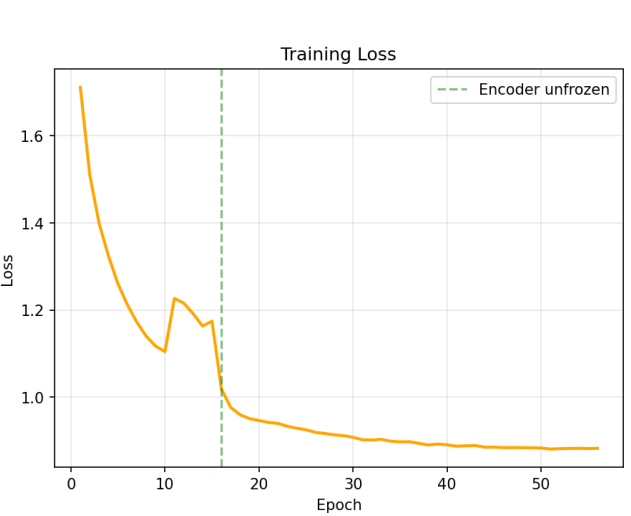
\includegraphics[width=\textwidth]{img/train_loss.png}
        \caption{Train loss vs Epoch}
        \label{fig:train_loss}
    \end{subfigure}
    \hfill                                              
    \begin{subfigure}[b]{0.48\textwidth}
        \centering
        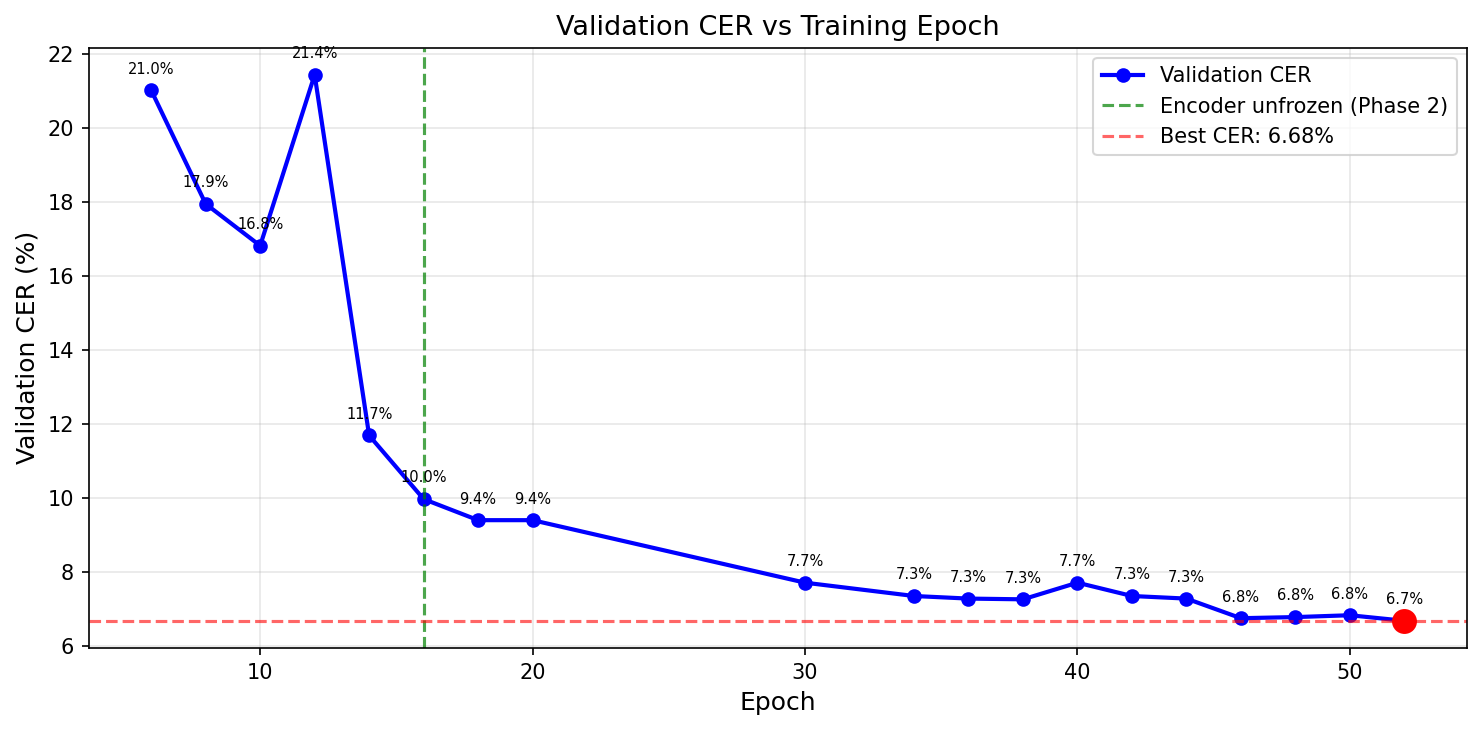
\includegraphics[width=\textwidth]{img/Val_cer.png} 
        \caption{Validation CER vs Epoch}
        \label{fig:val_cer}
    \end{subfigure}

    \caption{Training dynamics across epochs. The green dashed line marks the transition to Phase 2 (encoder unfrozen). The red dashed line indicates the best validation CER of 6.68\%.}
    \label{fig:training_curves}
\end{figure}


\newpage
\noindent The distribution of Normalized Edit Distance (NED) is highly right-skewed, indicating that the model performs very well on the majority of test samples while struggling with a small subset of more difficult cases. A total of 10,736 samples, representing approximately 83.5\% of the test set, achieved perfect recognition (NED = 0). This large concentration at zero demonstrates that the model is able to accurately predict most words without any character-level errors.

\noindent Despite this strong performance, the mean NED is 5.22\%, which is slightly elevated due to a small number of challenging samples forming a long, sparse tail in the distribution. These outliers correspond to cases where the model makes significant errors, including instances where predictions are entirely incorrect (NED = 100\%). However, such cases are relatively rare and do not substantially affect the overall performance trend.

\noindent Normalized Edit Distance is defined as the edit distance divided by the maximum length of the predicted and reference sequences. Unlike Character Error Rate (CER), which normalizes only by the reference length, NED accounts for both insertions and deletions more symmetrically by penalizing predictions that are excessively longer or shorter than the ground truth. In this evaluation, the NED (5.22\%) and CER (5.82\%) values are very close, suggesting that the model maintains good control over sequence length. In other words, it is neither frequently generating extra characters nor truncating outputs, which indicates stable and well-calibrated predictions.

\noindent Overall, the distribution reflects a model that is highly accurate on most inputs, with only a small proportion of difficult cases contributing to the residual error.
\begin{figure}[H]
    \centering
    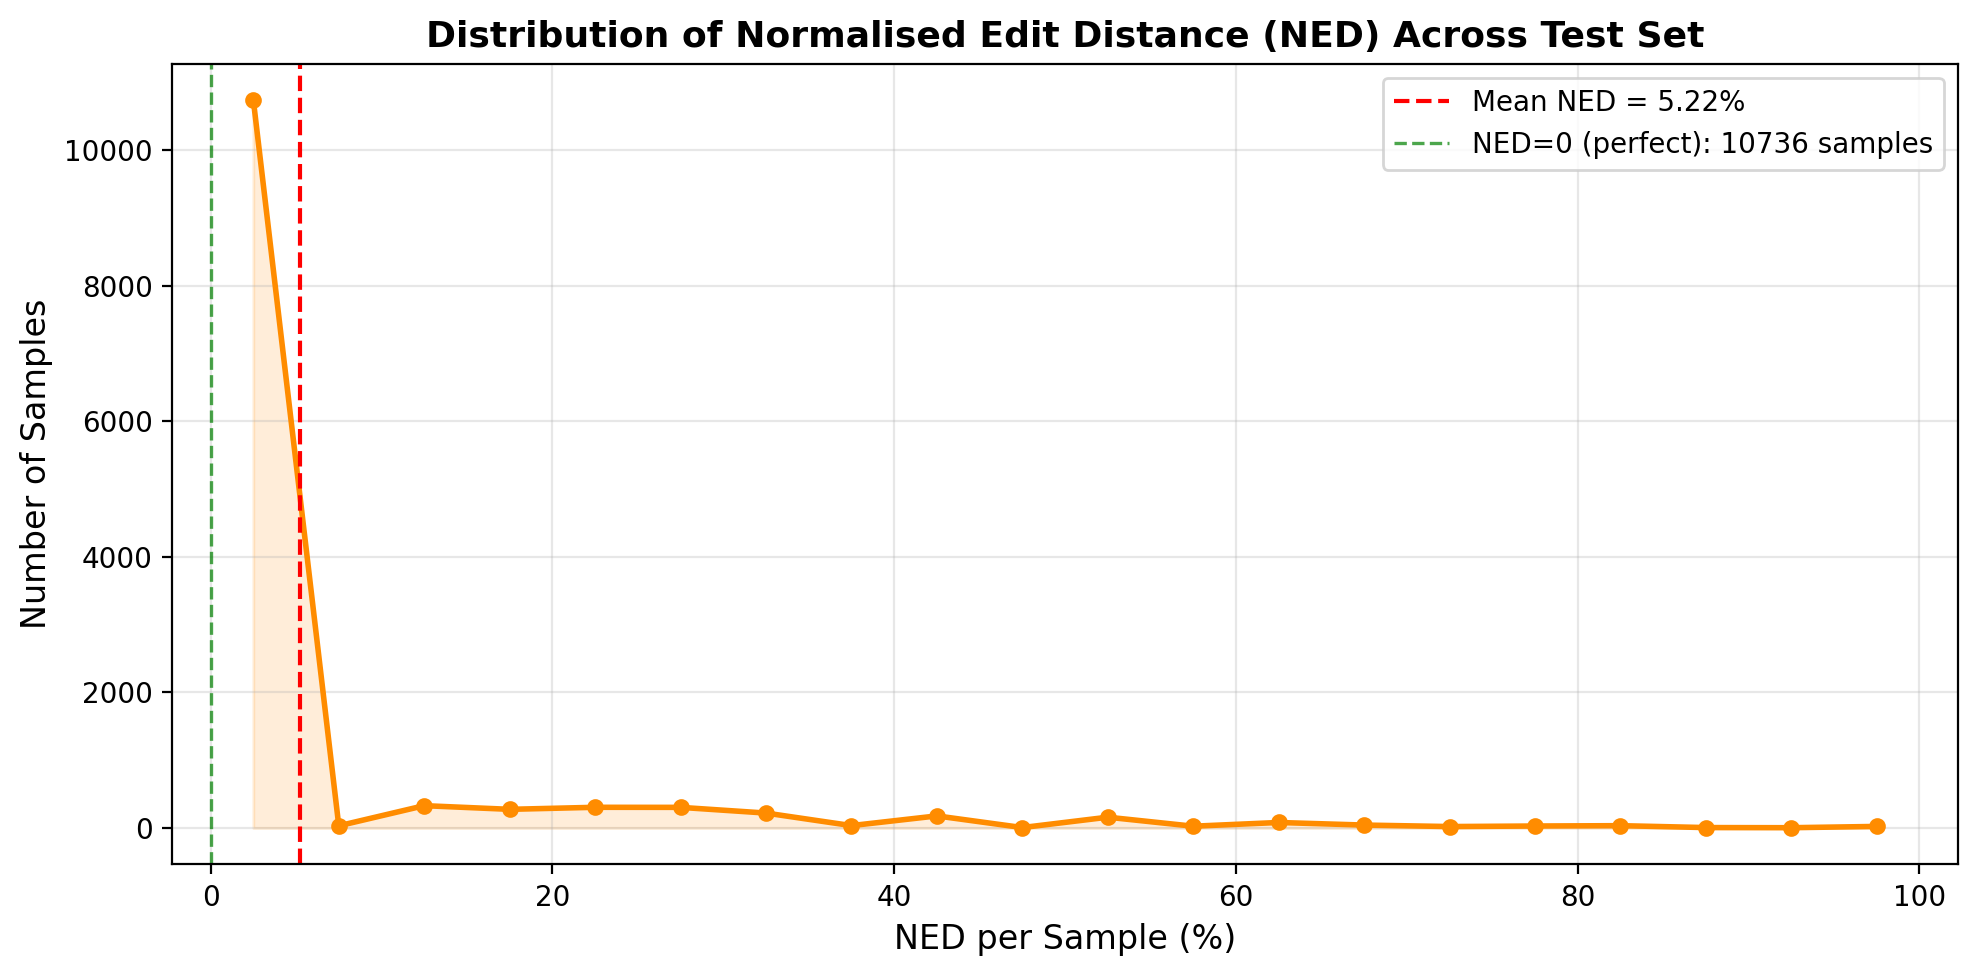
\includegraphics[width=0.85\textwidth]{img/metric_ned_distribution.png}
    \caption{Distribution of Normalised Edit Distance (NED) scores across the test set.}
    \label{fig:ned_dist}
\end{figure}
\newpage
\noindent Similarly, the cumulative accuracy analysis shows a steep and consistent improvement as the tolerance for character-level errors increases. At zero tolerance (K = 0), 83.5\% of the predictions are exactly correct, indicating a strong baseline performance. When a tolerance of one character error is allowed (K = 1), the accuracy rises significantly to 92.4\%, and further increases to 98.1\% by K = 3. Overall, the accuracy reaches 96.0\% within just two character errors, demonstrating that the majority of model predictions are very close to the ground truth.

\noindent This trend indicates that most of the model’s errors are minor, typically involving only one or two incorrect characters, rather than large or completely incorrect predictions. Such behavior suggests that the model is generally reliable and rarely produces catastrophic errors.

\noindent From an application perspective, this is a particularly strong result. In practical OCR systems integrated with downstream natural language processing tasks, small character-level errors are often recoverable through post-processing techniques such as spell-checking or language model correction. Therefore, even when the model does not achieve perfect predictions, its outputs remain highly usable and can be refined further with minimal effort.
\begin{figure}[H]
    \centering
    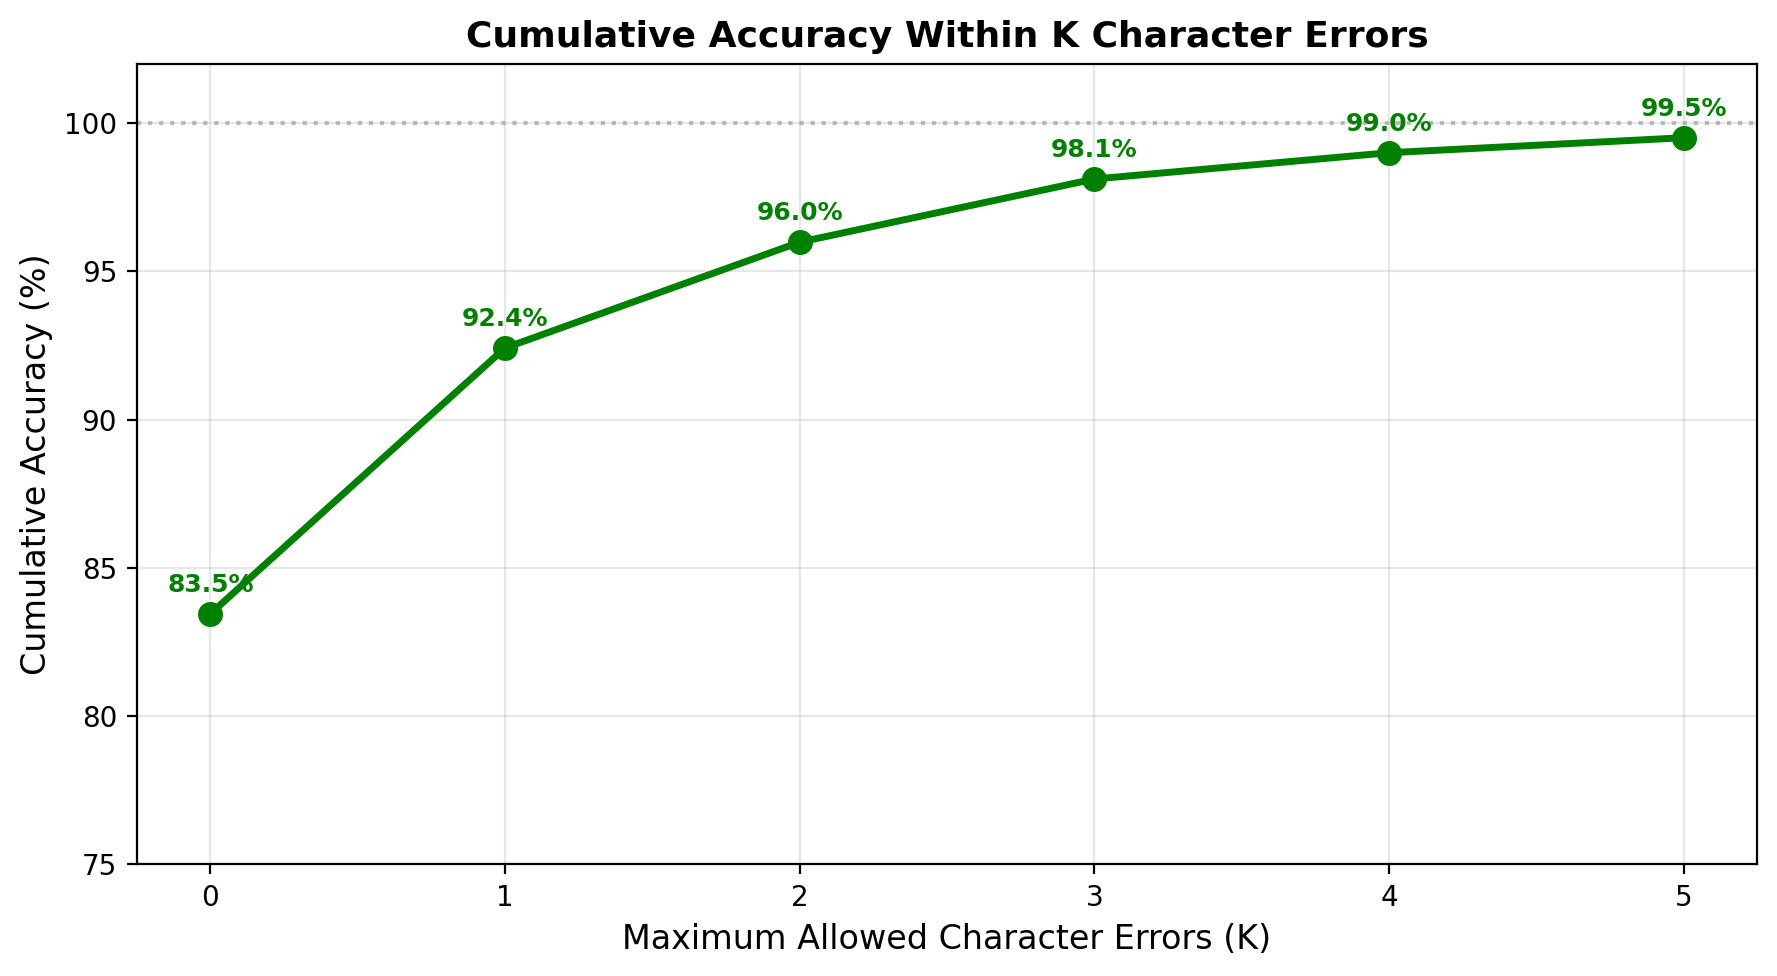
\includegraphics[width=0.85\textwidth]{img/metric_cumulative_accuracy.png}
    \caption{Cumulative accuracy within $K$ character errors.}
    \label{fig:cumulative_acc}
\end{figure}
\newpage
\noindent The evaluation of model performance across varying word lengths indicates that exact match accuracy remains relatively stable, ranging between 82\% and 85\% for words comprising 2 to 11 characters. In contrast, the Character Error Rate (CER) exhibits a pronounced decline as word length increases. This inverse relationship reflects the reduced proportional impact of individual character errors in longer sequences, where isolated mistakes contribute less significantly to the overall error metric.

\noindent A consistent trend is observed for shorter to mid-length words (lengths 1–9), where CER decreases substantially from approximately 29\% to around 4\%. This behavior is expected, as longer words provide increased contextual and structural information, enabling more reliable pattern recognition. Conversely, shorter words, particularly those consisting of one or two characters, present limited contextual cues and are therefore more susceptible to misclassification.

\noindent Variations in performance at higher word lengths, specifically at lengths 13 and 15, can be attributed primarily to limited sample sizes. With only 34 and 14 samples respectively, these categories are highly sensitive to the influence of a small number of difficult instances, resulting in noticeable fluctuations in both accuracy and CER. A similar phenomenon is observed at length 14, where accuracy reaches 89.5\% based on a sample size of 38, likely reflecting a relatively less challenging subset of data rather than a consistent performance improvement.

\noindent Performance degradation for very short words is particularly evident at length 1, where the dataset contains only 24 samples. In addition to the limited sample size, the inherent visual ambiguity of isolated Devanagari characters contributes to this effect. Characters combined with vowel diacritics (matras) often exhibit similar visual structures, and in the absence of surrounding context, the model faces increased difficulty in disambiguating such cases.
\begin{figure}[H]
    \centering
    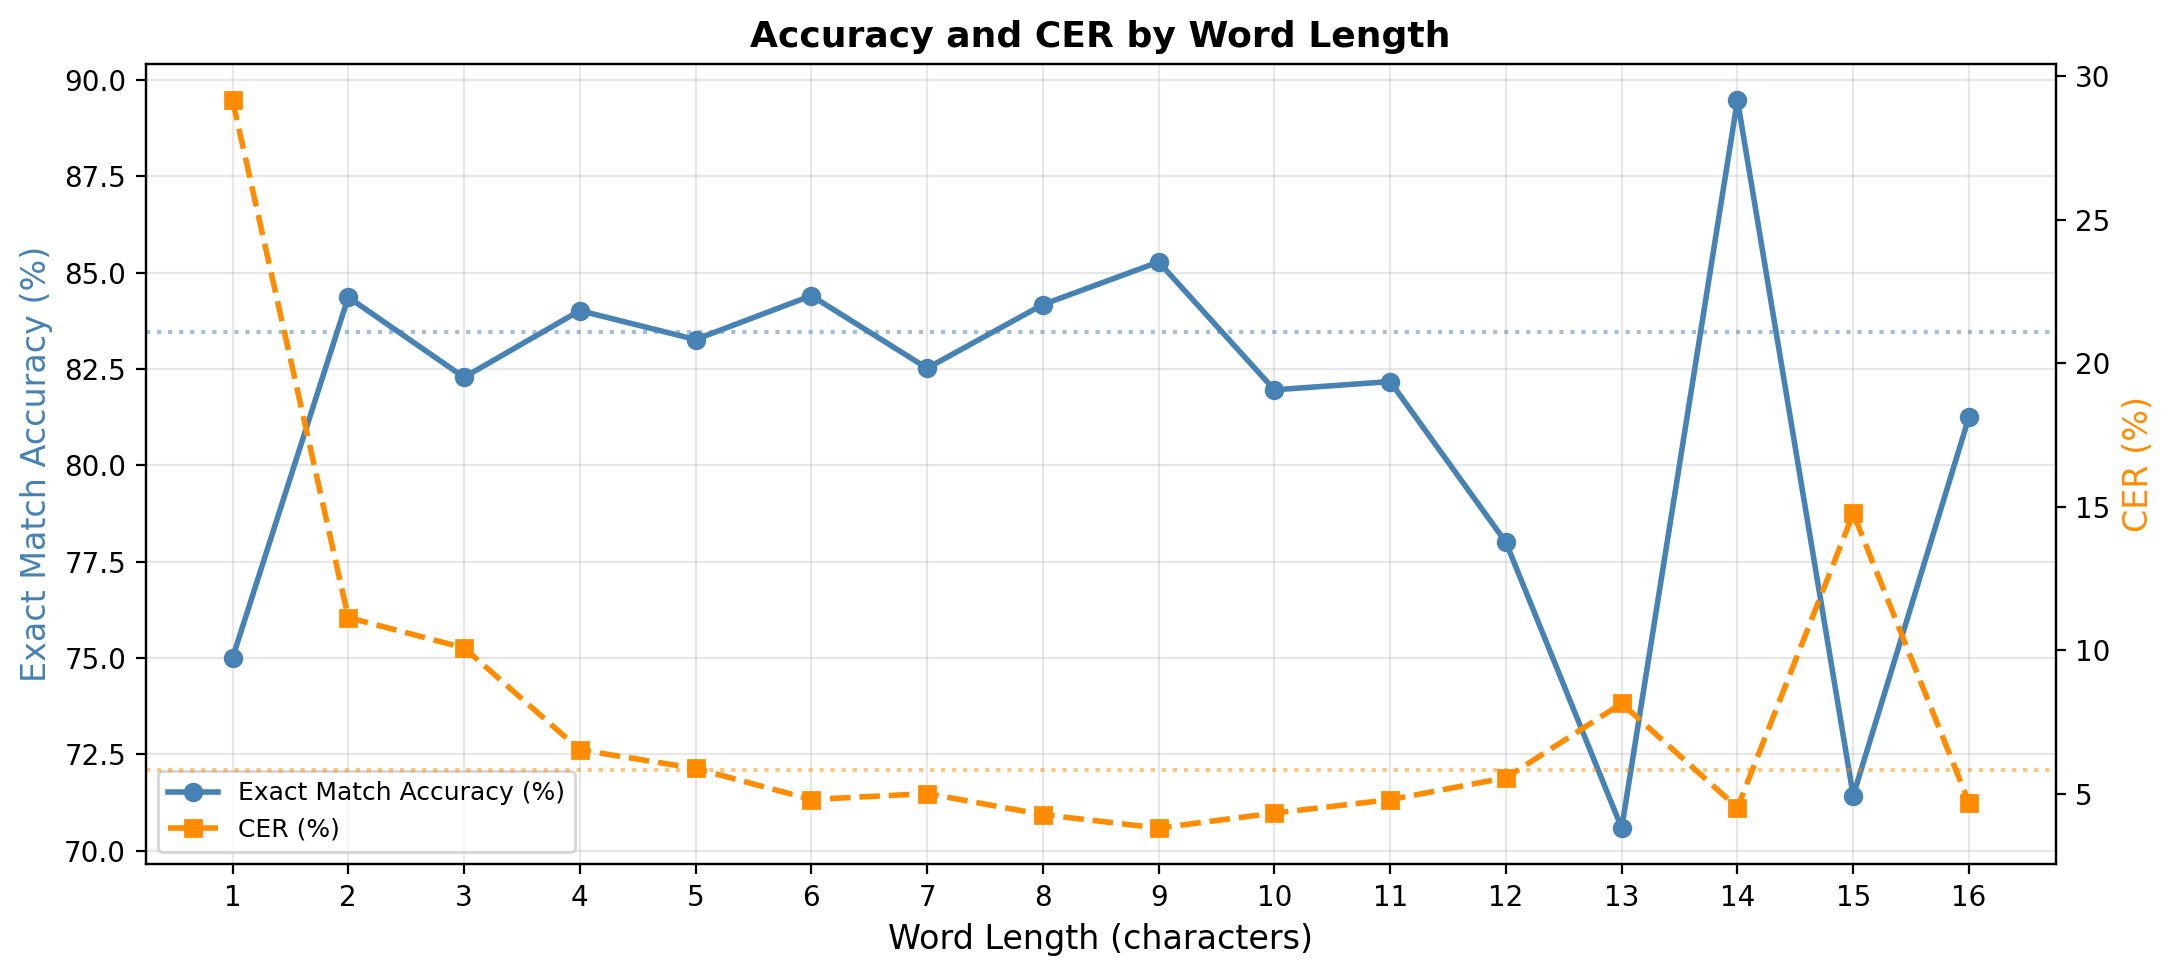
\includegraphics[width=0.85\textwidth]{img/metric_by_word_length.png}
    \caption{Exact Match Accuracy and CER as a function of word length.}
    \label{fig:by_length}
\end{figure}

\noindent Overall, The model achieves a CER of 5.82\%, WER of 16.55\%, NED of 5.22\%, exact-match accuracy of 83.45\%, and 1-NED of 94.78\%, collectively demonstrating strong character-level recognition with moderate word-level precision.
\begin{figure}[H]
    \centering
    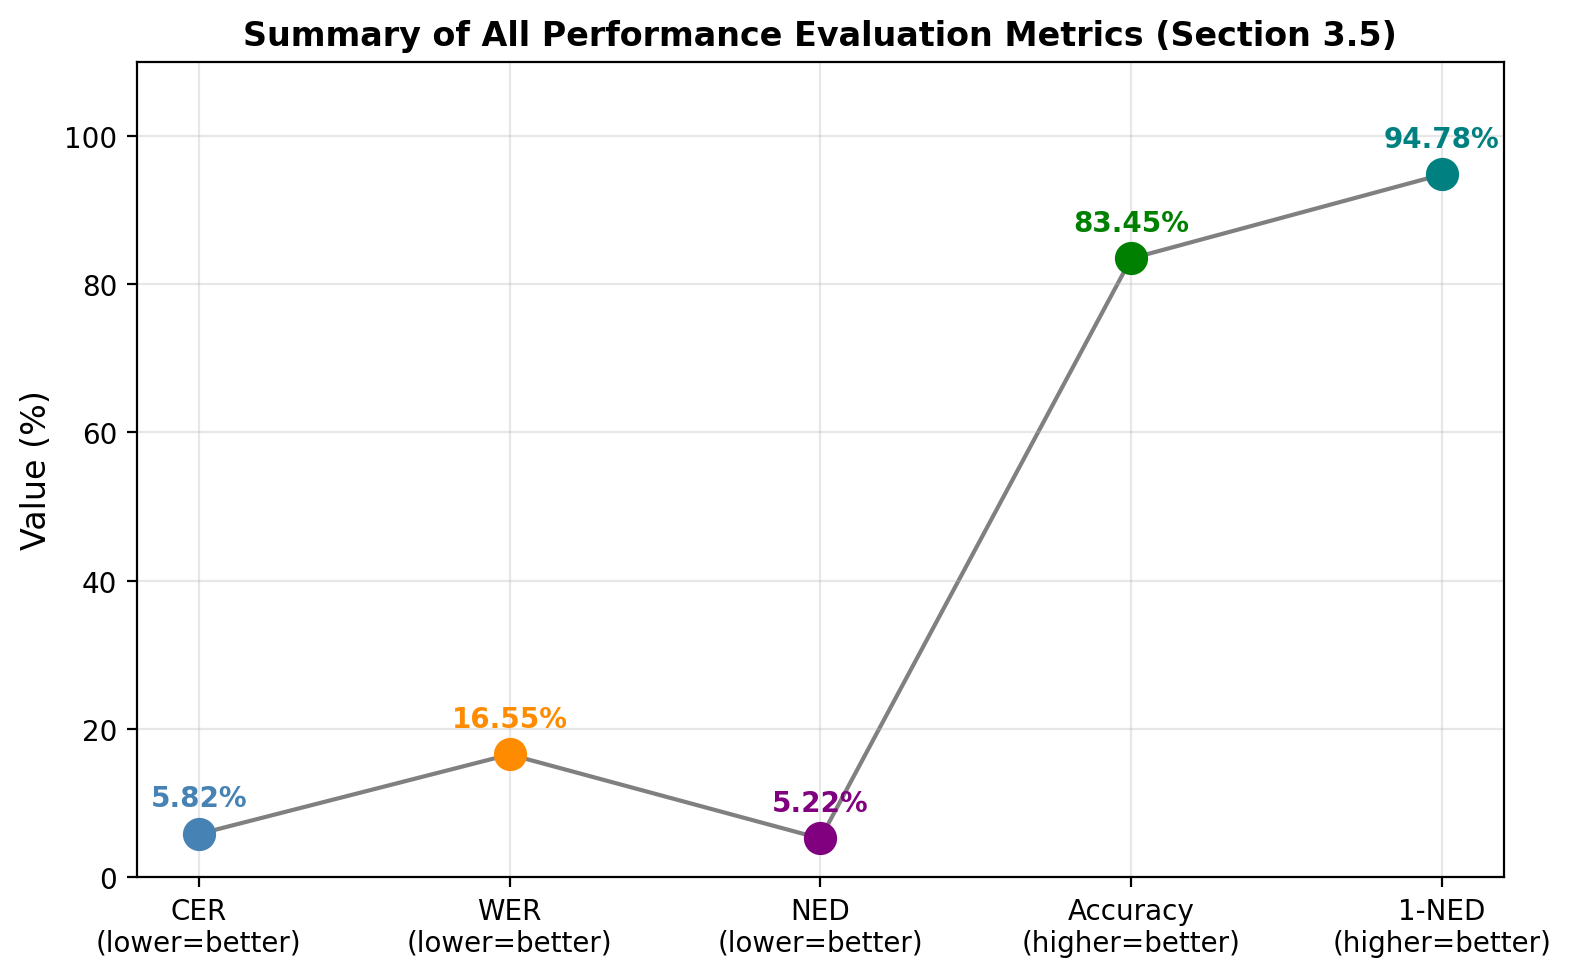
\includegraphics[width=0.75\textwidth]{img/metric_summary_all.png}
    \caption{Summary of all performance evaluation metrics (Section~3.5).}
    \label{fig:metric_summary}
\end{figure}


\newpage
\section{Software Development Approach}
\noindent Agile development methodology is a quick and flexible iterative development methodology for software development. It divides work into manageable chunks without requiring a lot of advance planning. The needs and scope of the project are established early on, and iterations are planned. A functioning product demo is the end result of each iteration, which includes all phases of the software development life cycle: planning, requirements analysis, design, coding, and testing. By iteratively improving the product in response to feedback, this methodology lowers project risk and speeds up delivery overall.
    \begin{figure}[H]
        \centering
        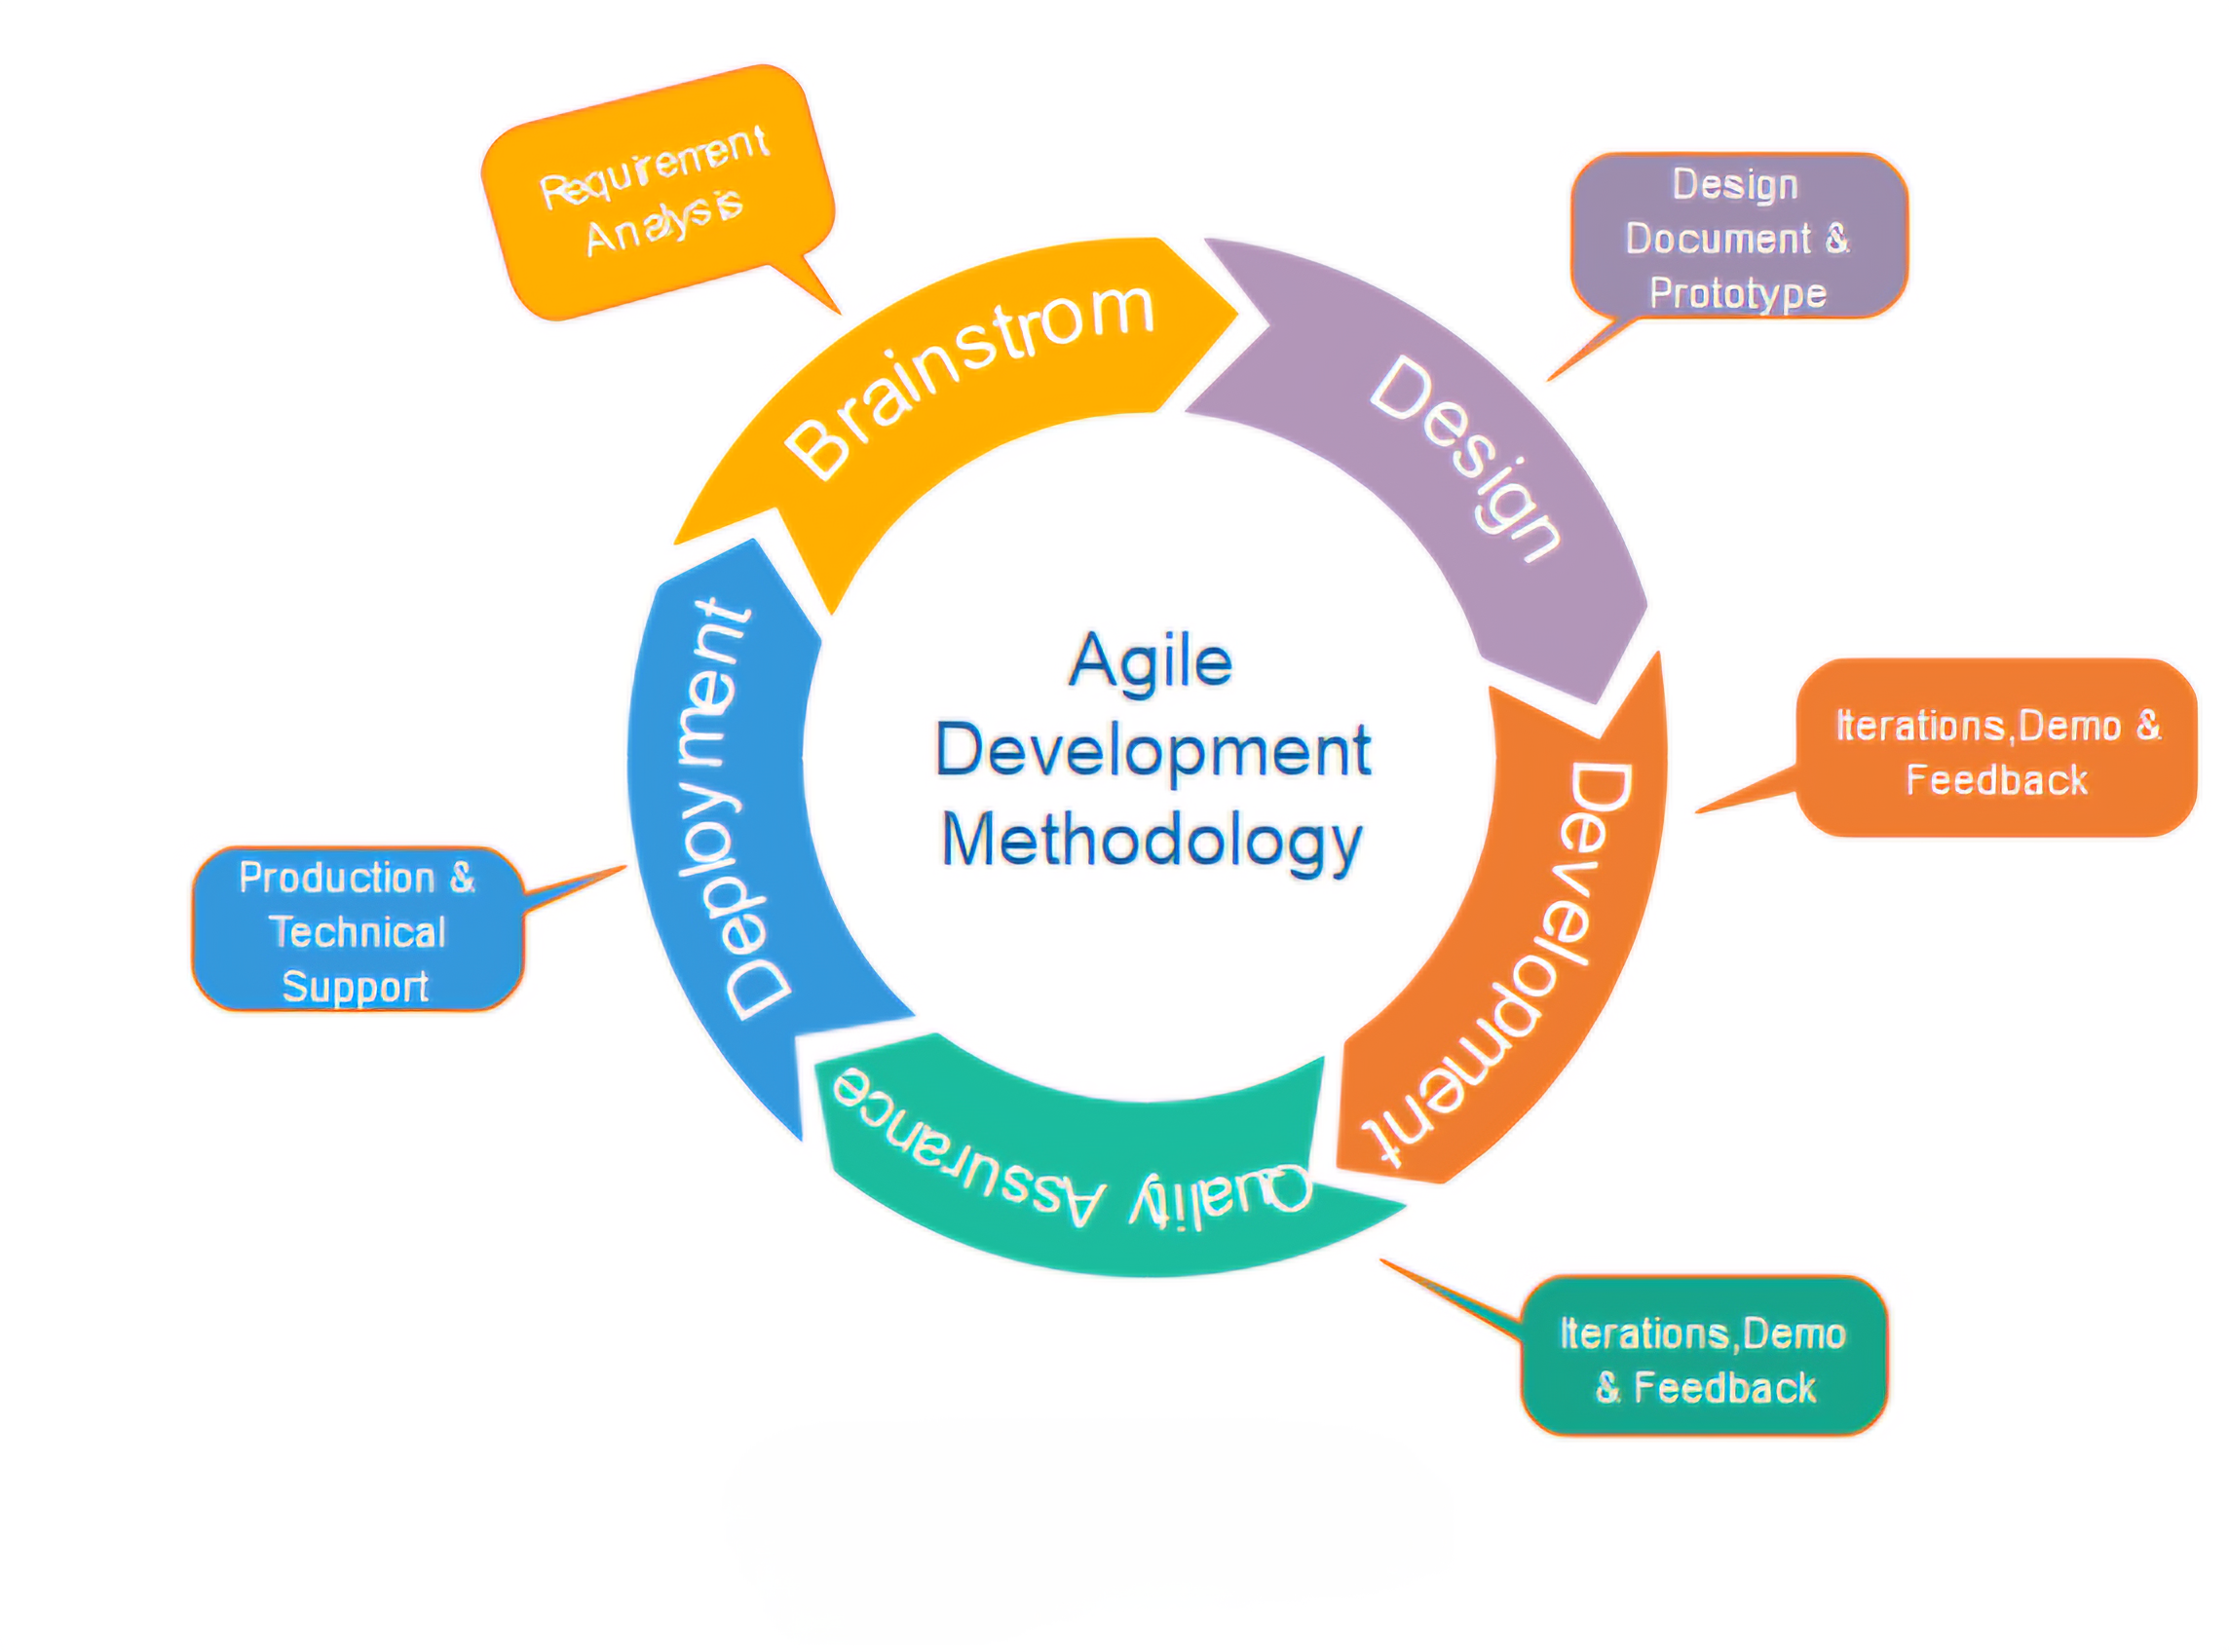
\includegraphics[scale=0.1]{img/agilemodel.png}
        \caption{Agile Development Model}
        \label{fig:agilemodel}
    \end{figure}
\subsection{Agile Sprints}

\subsubsection{Sprint 1: Dataset Acquisition and Initial Exploration}
\textbf{Duration:} Mid-December, Weeks 1--2\\
\textbf{Goal:} Identify and acquire a suitable dataset for handwritten Nepali word recognition and assess the feasibility of a character-level recognition approach.

\textbf{Key Activities:}
\begin{itemize}
    \item Surveyed publicly available Devanagari handwriting datasets and evaluated their suitability for word-level Nepali OCR.
    \item Acquired a Devanagari Character Dataset and manually curated 
    an additional matra (diacritic) dataset to supplement 
    underrepresented character classes.
    \item Implemented and tested an initial character-level recognition 
    pipeline to assess baseline feasibility.
    \item Identified critical limitations of the character-level 
    approach, including low accuracy and inadequate representation 
    of compound characters and matras.
    \item Collectively decided to abandon the character-level approach 
    in favour of word-level recognition based on evaluation outcomes.
\end{itemize}

\textbf{Outcomes:}
\begin{itemize}
    \item Character-level approach evaluated and rejected on accuracy 
    grounds.
    \item Decision made to adopt word-level recognition using a 
    dedicated word-image dataset.
    \item Clear direction established for Sprint 2.
\end{itemize}

\subsubsection{Sprint 2: Dataset Preparation and Pre-processing 
Pipeline}
\textbf{Duration:} Late December -- Early January, Weeks 3--5\\
\textbf{Goal:} Acquire the IIIT-HW-Dev word-level dataset, parse it 
into structured image--label pairs, and build a robust image 
pre-processing pipeline.

\textbf{Key Activities:}
\begin{itemize}
    \item Obtained the IIIT-HW-Dev dataset from Kaggle, comprising 
    95,380 segmented handwritten word images with Unicode labels, 
    and parsed it into training (69,802), validation (12,713), and 
    test (12,865) splits.
    \item Identified 108 unique Devanagari characters across the 
    dataset, with a maximum label length of 23 characters.
    \item Designed and implemented a multi-step image pre-processing 
    pipeline comprising grayscale conversion, Gaussian denoising, 
    adaptive binarisation, morphological closing, deskewing, tight 
    cropping, and letterbox padding to $128 \times 128$ pixels.
    \item Pre-cached all processed images to disk to avoid repeated 
    computation during training.
    \item Built and validated a custom character-level tokenizer with 
    a 112-token Devanagari vocabulary including four special tokens 
    (\texttt{<pad>}, \texttt{<s>}, \texttt{</s>}, \texttt{<unk>}).
\end{itemize}

\textbf{Outcomes:}
\begin{itemize}
    \item Fully parsed and split IIIT-HW-Dev dataset ready for 
    training.
    \item Pre-processing pipeline implemented, validated, and cached.
    \item Custom tokenizer built and smoke-tested on Devanagari 
    word samples.
\end{itemize}

\subsubsection{Sprint 3: Model Architecture Design and Initialisation}
\textbf{Duration:} January, Weeks 6--7\\
\textbf{Goal:} Design and initialise the encoder--decoder model 
architecture and configure the training infrastructure.

\textbf{Key Activities:}
\begin{itemize}
    \item Selected microsoft/trocr-base-handwritten as the 
    source of the pre-trained ViT encoder, leveraging its existing 
    fine-tuning on handwritten document images.
    \item Designed a lightweight custom BERT-based decoder with 2 transformer layers, 4 attention heads, hidden size 256, and FFN intermediate size 512 with approximately 4 million parameters that were sized appropriately for the training corpus.
    \item Integrated the encoder and decoder into a single end-to-end trainable model using HuggingFace's 
 VisionEncoderDecoderModel framework.
    \item Configured cross-attention between encoder and decoder, 
    token special IDs, and the data loading pipeline with on-the-fly 
    training augmentation (Gaussian blur, random affine, colour 
    jitter, random perspective, and random erasing).
    \item Set up mixed-precision training (fp16), gradient 
    accumulation over 4 steps, and automatic checkpoint uploading 
    to Kaggle every 2 epochs.
\end{itemize}

\textbf{Outcomes:}
\begin{itemize}
    \item Full model architecture designed and initialised.
    \item Training infrastructure configured and validated on a 
    small batch of training data.
    \item Data pipeline with augmentation confirmed operational.
\end{itemize}

\subsubsection{Sprint 4: Phase 1 Training -- Decoder-Only}
\textbf{Duration:} January -- February, Weeks 8--10\\
\textbf{Goal:} Train the decoder in isolation with the encoder frozen 
to establish baseline Devanagari text generation capability without 
disturbing pre-trained visual features.

\textbf{Key Activities:}
\begin{itemize}
    \item Froze all ViT encoder parameters and trained only the 
    decoder using AdamW with learning rate $5 \times 10^{-4}$ and 
    weight decay $10^{-3}$.
    \item Applied label-smoothed cross-entropy loss with smoothing 
    coefficient 0.1 and gradient clipping at norm 1.0.
    \item Monitored validation CER and WER every 2 epochs and saved 
    the best-performing checkpoint automatically.
    \item Observed steady reduction in validation CER across 
    training epochs, confirming that the decoder was successfully 
    learning Devanagari character generation patterns.
\end{itemize}

\textbf{Outcomes:}
\begin{itemize}
    \item Stable decoder-only baseline established.
    \item Best Phase 1 checkpoint saved for use in Phase 2.
    \item Validation CER and WER trends reviewed collectively to 
    inform Phase 2 training configuration.
\end{itemize}

\subsubsection{Sprint 5: Phase 2 Training -- Full Fine-Tuning}
\textbf{Duration:} February -- March, Weeks 11--14\\
\textbf{Goal:} Unfreeze the ViT encoder and fine-tune the entire 
model end-to-end to adapt visual features to handwritten Devanagari 
and further reduce CER.

\textbf{Key Activities:}
\begin{itemize}
    \item Unfroze the encoder and applied differential learning 
    rates: $5 \times 10^{-7}$ for the encoder and $5 \times 
    10^{-5}$ for the decoder, to prevent catastrophic forgetting 
    of pre-trained visual representations.
    \item Continued training with \texttt{CosineAnnealingWarmRestarts} 
    scheduler ($T_0 = 10$, $\eta_{\min} = 10^{-8}$) across multiple 
    Kaggle sessions, resuming from the latest checkpoint each time.
    \item Iteratively reviewed validation CER and WER at the end of 
    each session and adjusted hyperparameters accordingly.
    \item Achieved a best validation CER of 7.26\% over the course 
    of full fine-tuning.
    \item Applied early stopping with patience of 10 validation 
    rounds to prevent overfitting.
\end{itemize}
\newpage
\textbf{Outcomes:}
\begin{itemize}
    \item Best model checkpoint achieving 6.68\% CER saved for 
    evaluation.
    \item Full training completed across 52 epochs with early 
    stopping.
    \item Model confirmed stable and non-overfitting based on 
    train--validation loss gap monitoring.
\end{itemize}

\subsubsection{Sprint 6: Evaluation and Inference}
\textbf{Duration:} March, Weeks 15--16\\
\textbf{Goal:} Conduct final evaluation on the held-out test set, 
implement single-image inference with confidence scoring, and 
prepare the system for demonstration.

\textbf{Key Activities:}
\begin{itemize}
    \item Loaded the best model checkpoint and evaluated it on the 
    full test set of 12,865 word images using beam search 
    (num\_beams = 4).
    \item Computed CER, WER, and Exact Match Accuracy on the test 
    set after Unicode NFC normalisation of all predicted and 
    ground-truth strings.
    \item Implemented single-image inference with test-time 
    augmentation (TTA) across four image variants and confidence 
    scoring from beam sequence log-probabilities.
    \item Validated predictions qualitatively on sample test images 
    and batch inference grids.
    \item Compiled training curves, CER history, and sample 
    prediction outputs for inclusion in the project report.
\end{itemize}

\textbf{Outcomes:}
\begin{itemize}
    \item Final test set CER, WER, and Exact Match Accuracy 
    reported.
    \item Single-image inference pipeline operational with 
    confidence scoring.
    \item System ready for demonstration and submission.
\end{itemize}

\newpage
\section{Model Deployment}
This section describes the deployment of the developed Nepali Word Digitizer
system, including frontend implementation, backend services, and integration of the
trained model for real-time inference.
\subsection{Frontend Development}
The frontend of the system was developed using HTML, CSS, and JavaScript, 
providing a clean and responsive single-page web interface without relying 
on any frontend framework. Key frontend components included:

\begin{itemize}
    \item A drag-and-drop upload zone and file browser for uploading 
    handwritten images in PNG, JPG, or JPEG formats.
    
    \item A live image preview displayed immediately after upload for user 
    confirmation.
    
    \item A recognition result display showing the recognized Unicode Nepali 
    word in large Devanagari text.
    
    \item A character-level breakdown panel showing each predicted character 
    with its confidence score as a percentage and a visual progress bar, 
    derived from per-token transition probabilities computed during beam 
    search decoding.
    
    \item An alternative predictions panel displaying the top 3 beam search 
    candidates ranked by sequence log-probability score. Each candidate is 
    clickable, allowing the user to select a more appropriate prediction if 
    the top result is incorrect. Upon selection, the main display and 
    character-level confidence panel update to reflect the chosen candidate.
    
    \item A pipeline log panel displaying processing metadata such as model 
    name, device, number of beams, and image dimensions.
    
    \item Options to download the recognized text as a .txt file 
    or copy it directly to the clipboard.
    
    \item Status messages and error notifications for invalid uploads or 
    failed inference.
\end{itemize}
\noindent Screenshots of the user interface are provided in \Appendices~\ref{app:C1}.

\subsection{Backend Development}
The backend API was built using FastAPI, a modern Python web framework, and 
served the frontend directly. The backend development was primarily focused 
on the implementation and deployment of the deep learning model and its 
supporting components:

\begin{itemize}
    \item \textbf{TrOCR Model:} A Vision Encoder-Decoder model was 
    implemented for handwritten Nepali word recognition. The architecture 
    combines a Vision Transformer (ViT) encoder, pre-trained on Microsoft's 
    TrOCR base handwritten model, with a custom lightweight BERT decoder 
    consisting of 2 layers, 4 attention heads, and a hidden size of 256. 
    The model was fine-tuned on handwritten Nepali word images using a 
    custom Nepali tokenizer trained on Devanagari vocabulary.
    
    \item \textbf{Preprocessing Pipeline:} A dedicated preprocessing module 
    was implemented to prepare input images before inference. The pipeline 
    performs grayscale conversion, Gaussian blur denoising, adaptive 
    threshold binarization, morphological closing, deskewing, tight cropping 
    to the ink region, and letterbox padding to a fixed $128 \times 128$ 
    square before converting back to RGB for the model processor.
    
    \item \textbf{Configuration Management:} A centralized configuration 
    module was implemented to manage all system parameters including server 
    port, model and tokenizer paths, decoder architecture constants, and 
    generation hyperparameters. Parameters can be overridden at runtime via 
    environment variables without modifying source code.
\end{itemize}

The trained model and tokenizer were loaded during application startup using 
PyTorch's model loading mechanism, keeping them in memory throughout the 
runtime to ensure fast inference on subsequent requests. Supporting backend 
functionalities included:

\begin{itemize}
    \item Loading and initializing the TrOCR model and Nepali tokenizer at 
    startup.
    
    \item Receiving and reading uploaded image files via multipart form data 
    with validation for unsupported file types.
    
    \item Preprocessing input images through the image preparation pipeline.
    
    \item Running model inference using beam search decoding and converting 
    generated token IDs to Unicode Nepali text using the custom tokenizer.
    
    \item Computing per-character confidence scores from token transition 
    probabilities for all returned sequences.
    
    \item Returning the top 3 alternative predictions, each with its 
    sequence-level log-probability score and per-character confidence 
    breakdown.
    
    \item Error handling during file reading, preprocessing, and model 
    inference.
\end{itemize}

\subsection{Model Integration}
Once the model, preprocessing pipeline, and frontend interface were 
implemented and tested individually, the final phase involved full system 
integration:

\begin{itemize}
    \item Uploaded images are received by the FastAPI backend and passed 
    through the preprocessing pipeline.
    
    \item The cleaned image is processed by the TrOCR processor to generate 
    pixel tensors.
    
    \item The fine-tuned model performs beam search decoding to generate token IDs, which are decoded into Unicode Nepali text using the custom tokenizer.
    
    \item The top 3 candidate predictions are returned alongside their 
    sequence-level log-probability scores. Per-character confidence scores 
    are computed from token transition probabilities for each candidate 
    sequence.
    
    \item The recognized word, alternative candidates, character-level 
    confidence breakdown, and pipeline metadata are returned as a JSON 
    response and rendered on the web interface, where users can review and 
    select an alternative prediction if needed.
\end{itemize}

This end-to-end integration provided a smooth and accessible experience for 
handwritten Nepali word digitization, combining deep learning, image 
processing, and web technologies into a single functional application. By 
following Agile principles, such as iterative development and continuous 
feedback, we were able to build a reliable and functional word recognizer 
using modern deep learning and lightweight deployment technologies.
    \chapter{CONCLUSION}
\label{ch:conclusion}

\section{Objectives Achieved}
\label{sec:objectivesachieved}

The objective stated in Section~\ref{sec:objectives} names four things the system was to do. Table~\ref{tab:objachieved} takes each in turn and states what was delivered against it.

\begin{table}[htbp]
    \centering
    \caption{Each objective, what was delivered against it}
    \label{tab:objachieved}
    \small
    \setlength{\tabcolsep}{4pt}
    \begin{tabularx}{\textwidth}{|p{4.2cm}|Y|}
        \hline
        \textbf{Objective} & \textbf{What was delivered}\\
        \hline
        Establish the signed form of six NSL emergency phrases with NSL experts
        & Two in-person consultations, at the Rehabilitation Centre for the Rural Deaf and the National Federation of the Deaf Nepal. The form of each phrase was fixed and recorded before any data was collected, and phrase 6 was changed on the consultants' advice.\\
        \hline
        Build a custom landmark-based dataset from multiple signers
        & 840 clips from eight signers across seven classes, balanced at exactly 120 per class. Landmarks only; no video of any signer was stored.\\
        \hline
        Train and evaluate a BiLSTM classifier on signers absent from training
        & Eight leave-one-signer-out folds giving 95.18\% mean accuracy ($\pm$1.74) and 95.36\% pooled, with per-class F1 between 0.946 and 0.988 on the six phrases. Achieved, and it is the primary contribution of this work.\\
        \hline
        Deploy in a mobile application that recognises on-device and outputs text and speech
        & An Android application carrying a TensorFlow Lite model verified against the original to $1.2 \times 10^{-7}$. Recognition runs end to end on a physical device with the network disabled, displaying the phrase in Nepali and English and speaking it in Nepali.\\
        \hline
    \end{tabularx}
\end{table}

\noindent Every clause of the objective was met. The one qualification, which belongs with the fourth row rather than against it, is that the accuracies in the third row were measured on the recorded landmark path and not on the deployed one. The application runs; what it scores as installed has not been measured. That is the first limitation below and the first item of future work.

\section{Conclusion}

This project built a working recogniser for six Nepali Sign Language emergency phrases and delivered it as an Android application that displays the recognised phrase and speaks it in Nepali.

Two outputs will outlast the application. The first is the dataset. No public collection of NSL emergency phrases existed at the start of this work. The signed form of every phrase in this one was established in person with Deaf experts before any recording began, so it records real NSL rather than an approximation. The second is the evaluation protocol. Every clip carries the identity of the person who recorded it, and every accuracy reported here was produced by a model trained without that person. That gives 95.18\% mean across eight folds and 95.36\% pooled, against 97.62\% for the same architecture under a random split. The 2.3-point difference is a measurement of how much a random split flatters a model when clips from one person sit on both sides of it. Published NSL results are generally reported without this separation, so the lower figure is the one that any future work adopting the same protocol can be compared against.

The method is what made a dataset of this size sufficient. Each frame is reduced to a 225-value feature vector of pose and hand landmarks rather than pixels, normalised against the shoulder midpoint and each wrist, and standardised to 146 frames. A bidirectional LSTM of 192{,}007 parameters classifies the result and trains in minutes on a laptop processor. It exports to TensorFlow Lite at 881 kilobytes and runs on the phone that captured the frames, with no network connection at any point.

The system can also decline to answer. A seventh class trained on non-signing motion gives it somewhere to put an input that is not one of the six phrases, and a confidence threshold holds back anything the model is unsure of. For a tool whose output is a spoken emergency announcement, staying silent is worth as much as being right.

\section{Limitations}

The limitations fall into two kinds. The first three bound what the reported numbers mean. The remaining five bound what the system can do.

\subsection{Limitations on What the Numbers Mean}

\begin{enumerate}
    \item \textbf{The deployed accuracy has not been measured directly.} Every figure in this report was obtained on landmarks extracted by MediaPipe Holistic through a webcam. The phone uses a different extractor and a ported implementation of the preprocessing. The numbers therefore describe the method rather than the delivered application. The port is pinned to the original by generated fixtures, and two on-device distortions were found and corrected. But no experiment in this report establishes what the system scores as installed. This is the most consequential limitation in the list, and the measurement that would settle it is the first item of future work.

    \item \textbf{Eight signers, four of them the authors.} Every accuracy reported rests on eight people. The standard deviation across folds is 1.74 percentage points and the range is 5.7, so the estimate of performance on a new signer carries real uncertainty. Signers 01 to 04 are the four project members, who are not fluent NSL users and reproduced the consultants' reference performance. Signers 05 to 08 are the Deaf experts who set that reference. The reported accuracy is an accuracy on a mixture of fluent and learned signing, and the four author folds average 1.1 points above the other four.

    \item \textbf{The negative class is the weakest class.} Recall on \texttt{none} is 0.833, and twenty non-signs were classified as emergency phrases. Each is a case where the system would announce an emergency that nobody signed. These are just over half of all errors, and more than twice the nine cases in which one phrase is confused with another. The fix is a broader negative class rather than a stricter threshold, though how many of the twenty cleared the threshold has not been measured.
\end{enumerate}

\subsection{Limitations on What the System Can Do}

\begin{enumerate}
    \setcounter{enumi}{3}
    \item \textbf{Six phrases.} The vocabulary is fixed and small. A user with a need not on the list has no way to convey it.

    \item \textbf{One sign at a time.} The system recognises a single complete phrase per interaction. It does not segment continuous signing or handle more than one person in frame.

    \item \textbf{Facial expression is ignored.} The consultants confirmed no phrase in this set depends on it. The exclusion is safe for these six phrases and would not hold for a larger vocabulary.

    \item \textbf{Duration is only encoded below 146 frames.} Clips longer than the sequence length are uniformly subsampled, so signing longer than about 9.3 seconds is scale-normalised rather than measured.

    \item \textbf{Recognition speed depends on the phone.} Landmark extraction on a phone processor does not reach the capture rate of the training data, and the temporal resampling of Section~\ref{sec:ondevice} exists to absorb that. It restores the timescale but not the motion detail a low frame rate never sampled, so a slower device gives the model a coarser version of the same sign.
\end{enumerate}

\section{Future Work}

The first three items need no new recordings and could be carried out on the data and code that already exist. The remaining four require new data or new consultation, and are ordered by what they would buy.

\subsection{Immediate: No New Data Required}

\begin{enumerate}
    \item \textbf{Measure the on-device path against the recorded one.} Inference already runs on the phone, but with a different landmark extractor than the dataset was recorded with. No number in this report describes the installed system directly. The comparison that would fix this is implemented in the codebase and has not been run. It requires recording roughly 35 clips through both extraction paths at once, which isolates the landmark source from the signer, the framing, and the session, because the frames are the same. This is the correct next step: it either confirms the deployed accuracy or identifies what re-recording would cost.

    \item \textbf{Measure how often a false announcement clears the threshold.} The confidence carried by each of the twenty misclassified negatives is not recorded in the saved metrics. That number decides whether the threshold has anything left to give. Obtaining it needs no new data, only an extra column in the evaluation output.

    \item \textbf{Investigate the two directional phrase confusions.} Seven of the nine phrase-to-phrase errors fall on two pairs that leak in one direction only. \texttt{cant\_breathe} is read as \texttt{call\_police} and \texttt{need\_ambulance} as \texttt{building\_on\_fire}, never the reverse. A one-directional error is a clue rather than noise, since it suggests one signed form contains an opening the other shares. Reviewing the recordings of those four classes against the consultants' reference would establish whether the cause lies in the signs, in a subset of the signers, or in the representation. It costs review time rather than new data.
\end{enumerate}

\subsection{Requires New Recording or Consultation}

\begin{enumerate}
    \setcounter{enumi}{3}
    \item \textbf{Recruit more signers, prioritising fluent ones.} The clearest route to a more trustworthy accuracy figure is more people, and specifically more fluent NSL users. Doubling the signer count would narrow the confidence in the leave-one-signer-out estimate more than any change to the model. Section~\ref{sec:ablation} supports that ordering with a measurement rather than an argument: six architectures spanning a sevenfold range of parameter counts differ from one another by less than the spread between signers. Architecture search has little left to give; signer coverage has a great deal.

    \item \textbf{Broaden the negative class.} Recording more varied non-signing motion, targeted at the kind of motion the twenty misclassified clips resemble, is the direct route to reducing false announcements. It addresses just over half of the errors the system currently makes.

    \item \textbf{Extend the vocabulary.} The pipeline is not specific to these six phrases. Adding a phrase requires the consultation step, clip recordings, a spoken Nepali recording for the announcement, and a retrain, with no change to the preprocessing or the architecture.

    \item \textbf{Handle continuous signing.} Recognising a phrase within a stream, with no taps to mark its boundaries, is the main step from a proof of concept toward something usable without instruction.
\end{enumerate}


    % ── References ────────────────────────────────────────────────────────────
    \newpage
    \renewcommand{\bibname}{REFERENCES}
    \bibliographystyle{IEEEtran}
    \bibliography{reference}
    \addcontentsline{toc}{chapter}{REFERENCES}

    % ── Appendix ──────────────────────────────────────────────────────────────
    \clearpage
    \appendix
    % ================= Appendix A =================
\chapter{Field Consultation with NSL Experts}
\label{app:fieldwork}

The signed form of each of the six emergency phrases was established in person with Deaf experts before any data collection began, as described in Section~\ref{sec:phase0}. Consultations were held at the Rehabilitation Centre for the Rural Deaf in Bhaktapur and at the National Federation of the Deaf Nepal in Ranibari Marga, Samakhushi, Kathmandu. The images below are reproduced with the consent of those photographed.

\begin{figure}[H]
    \centering
    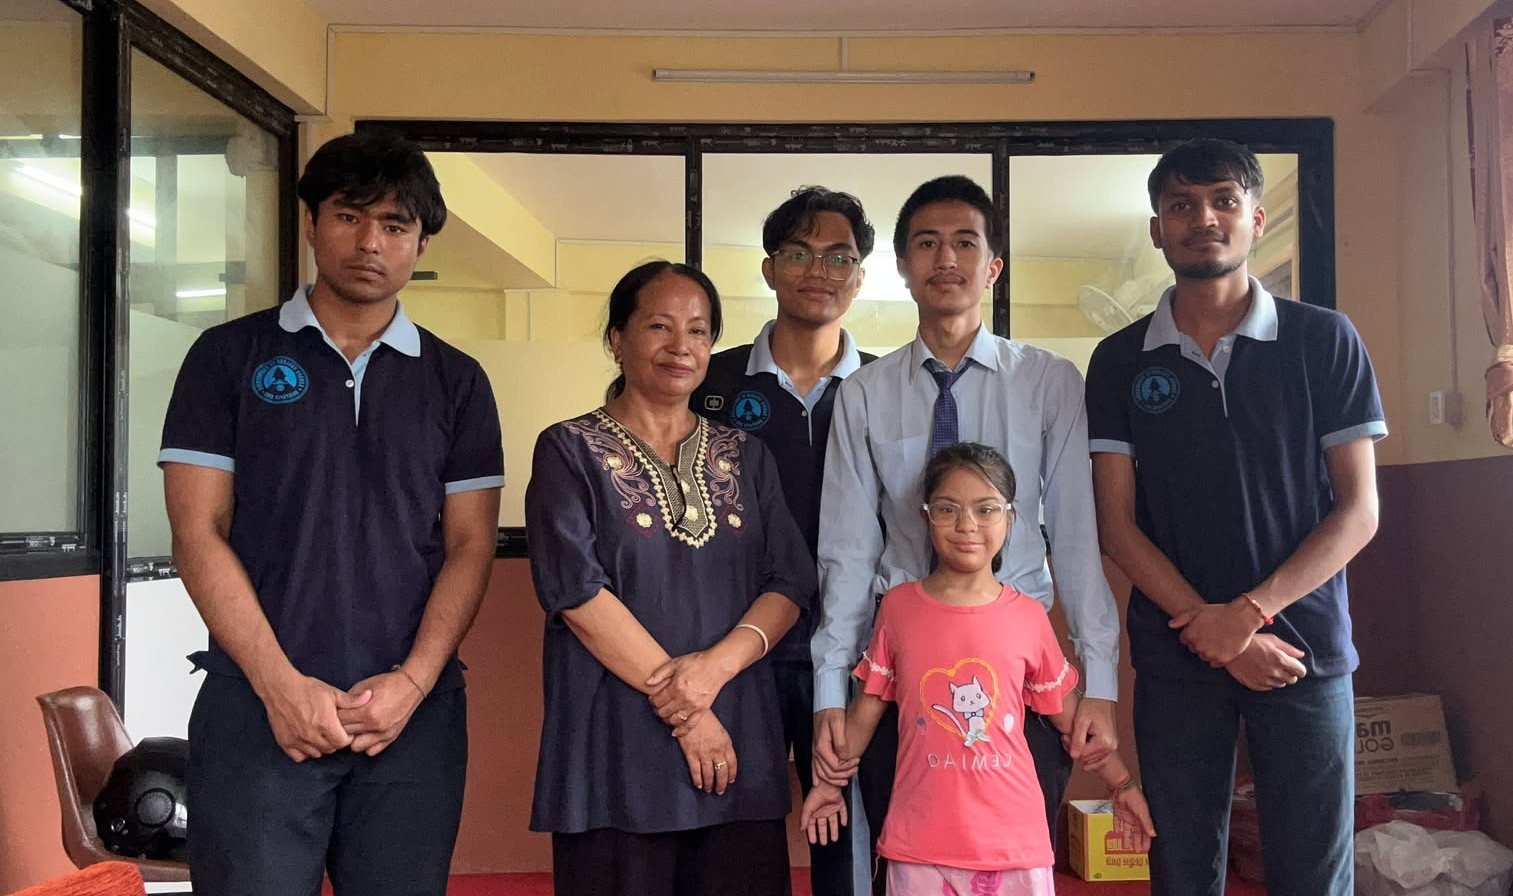
\includegraphics[width=0.72\textwidth]{img/consult1.jpg}
    \caption{The project team with the NSL consultant following a gloss consultation session}
    \label{fig:consult-group}
\end{figure}

\begin{figure}[H]
    \centering
    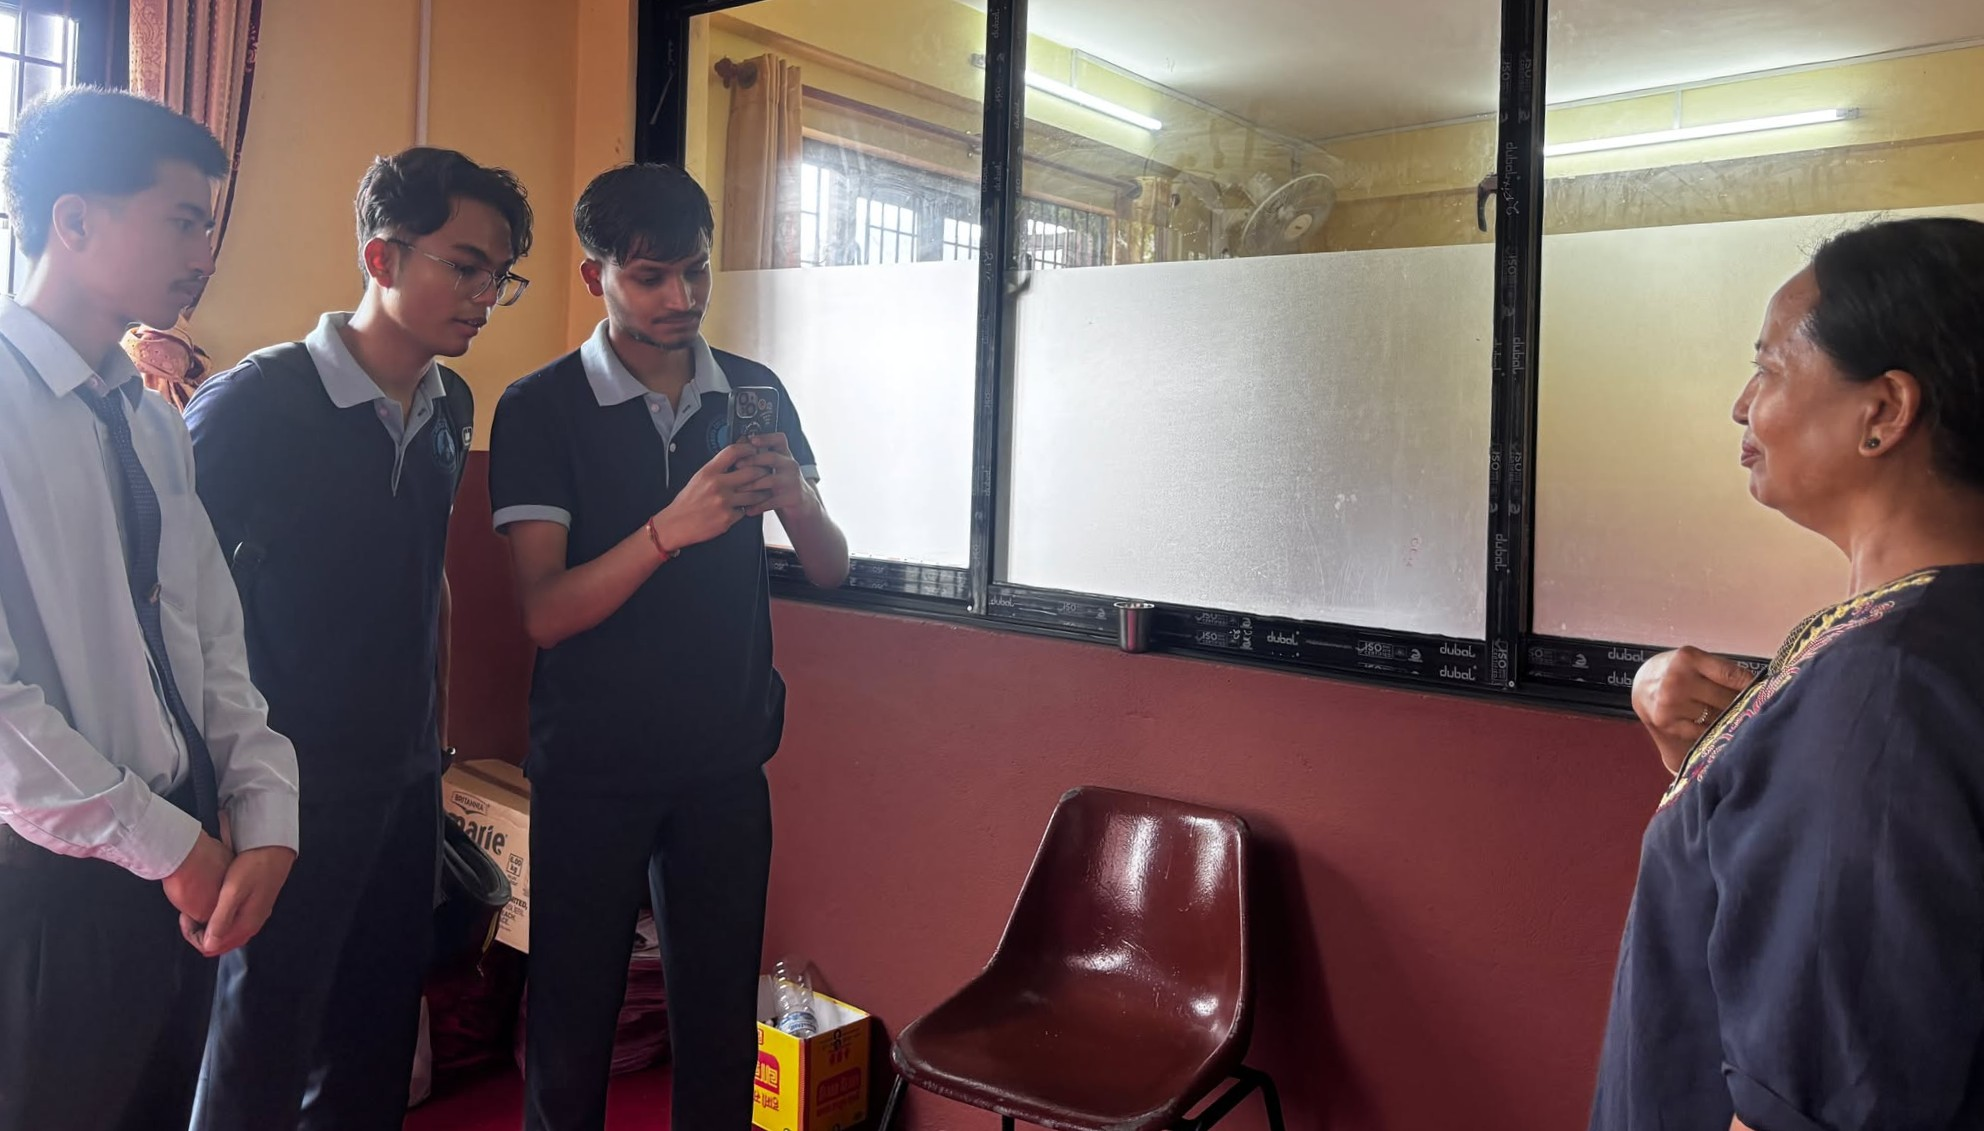
\includegraphics[width=0.72\textwidth]{img/consult2.jpg}
    \caption{Reviewing a recorded demonstration with the consultant to confirm the reference form of a phrase}
    \label{fig:consult-review}
\end{figure}

\begin{figure}[H]
    \centering
    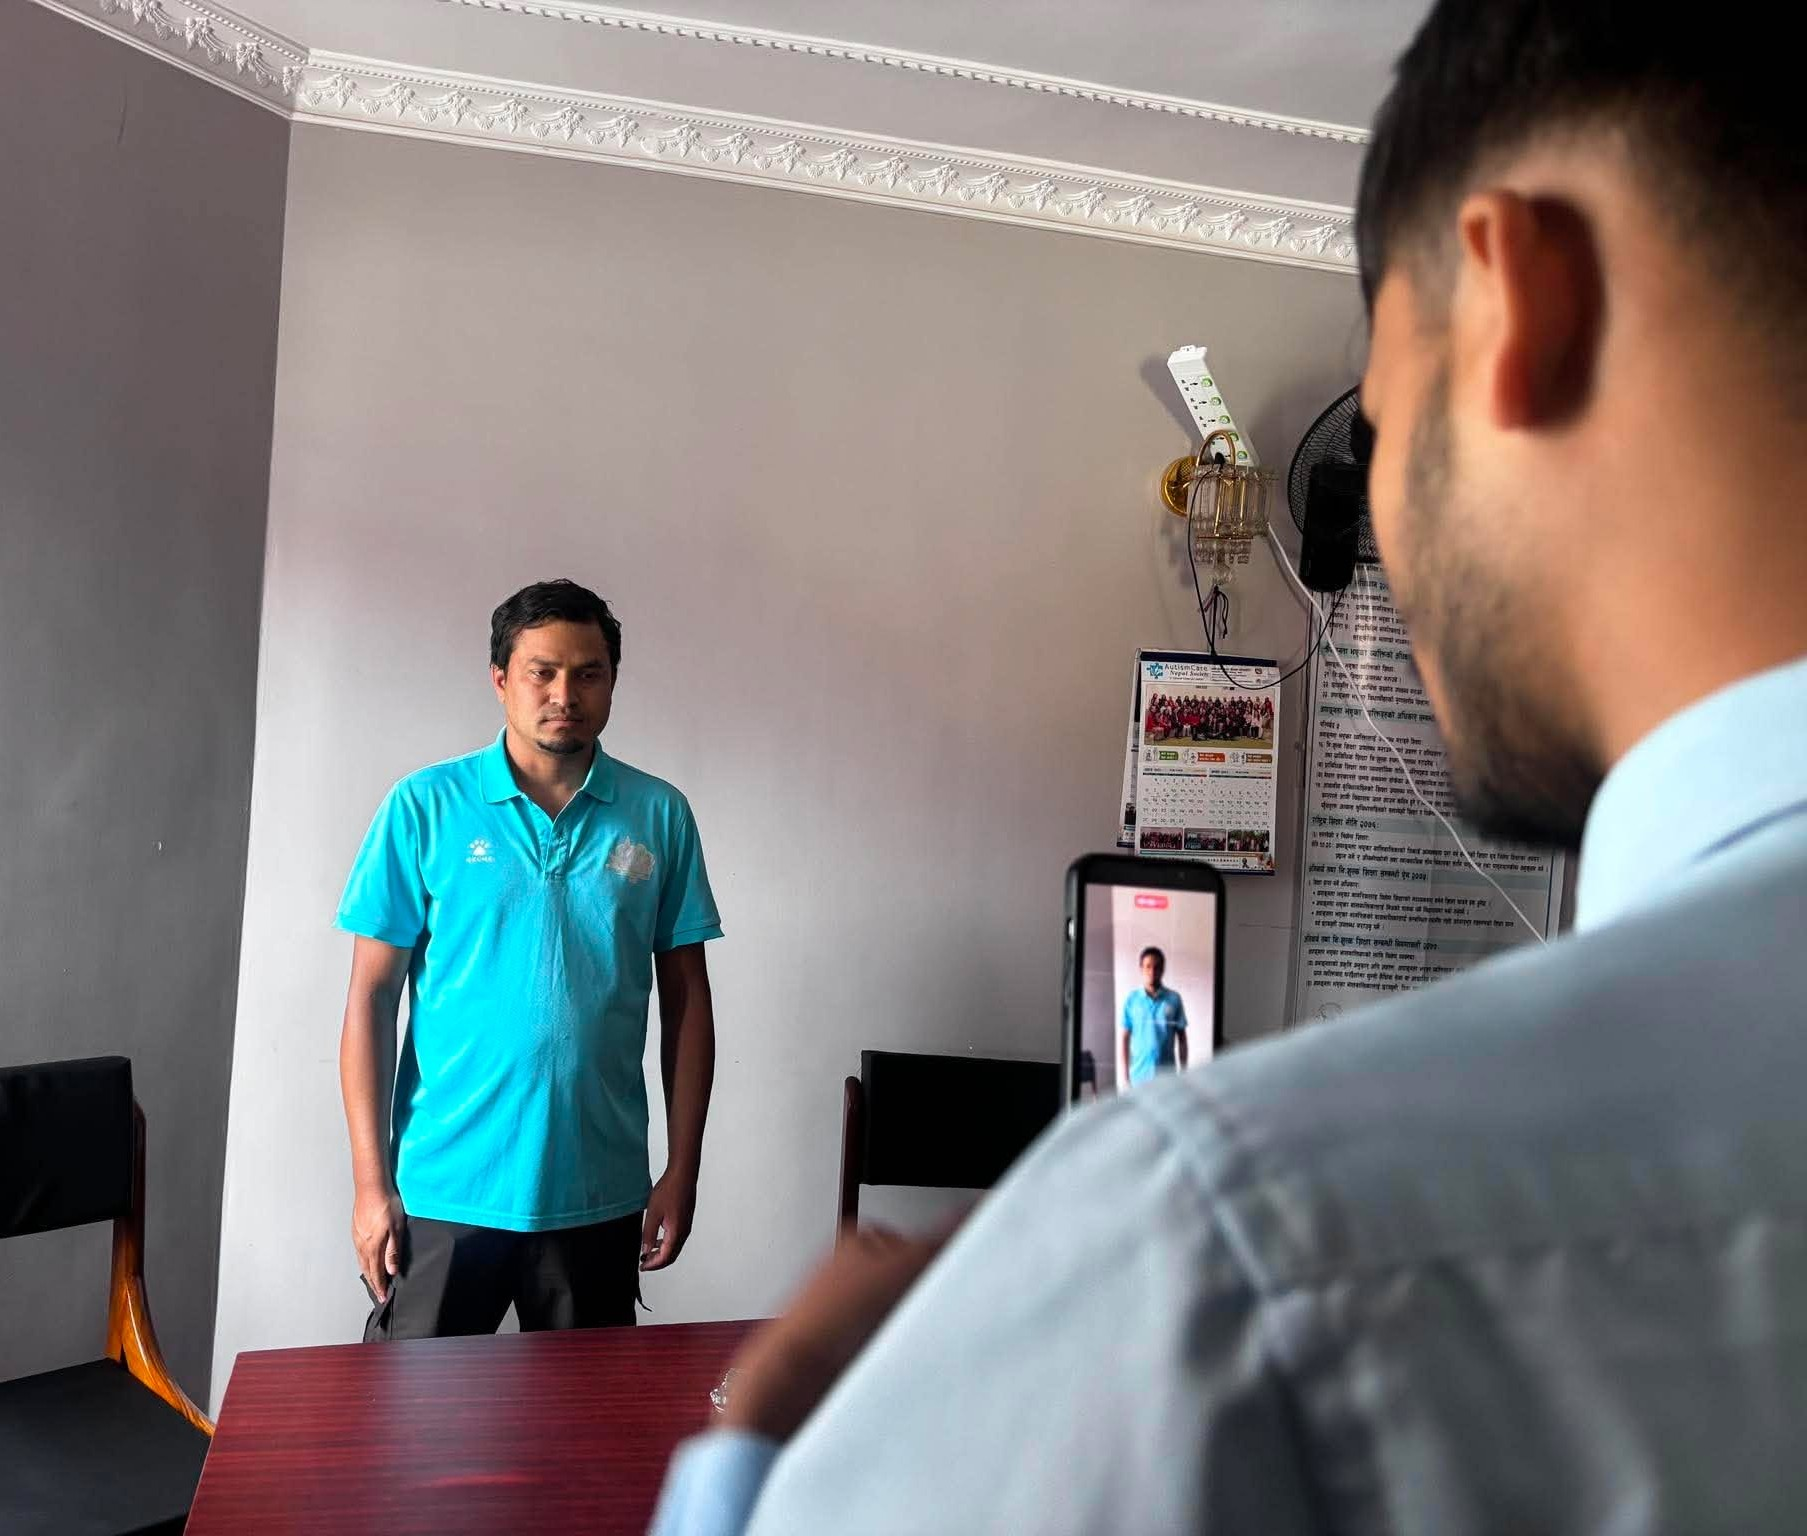
\includegraphics[width=0.72\textwidth]{img/consult3.jpg}
    \caption{An NSL expert demonstrating the signed form of a phrase for reference recording}
    \label{fig:consult-demo}
\end{figure}

% ================= Appendix B =================
\chapter{Data Collection Tool}
\label{app:recorder}

Clips were recorded with a purpose-built tool that runs MediaPipe Holistic on a live webcam feed and saves the 225-value landmark vector for each frame. The operator selects a signer identity and a phrase, then starts and stops each recording explicitly. Landmark overlays are drawn live, so a failed detection is visible during recording instead of afterwards.

\begin{figure}[H]
    \centering
    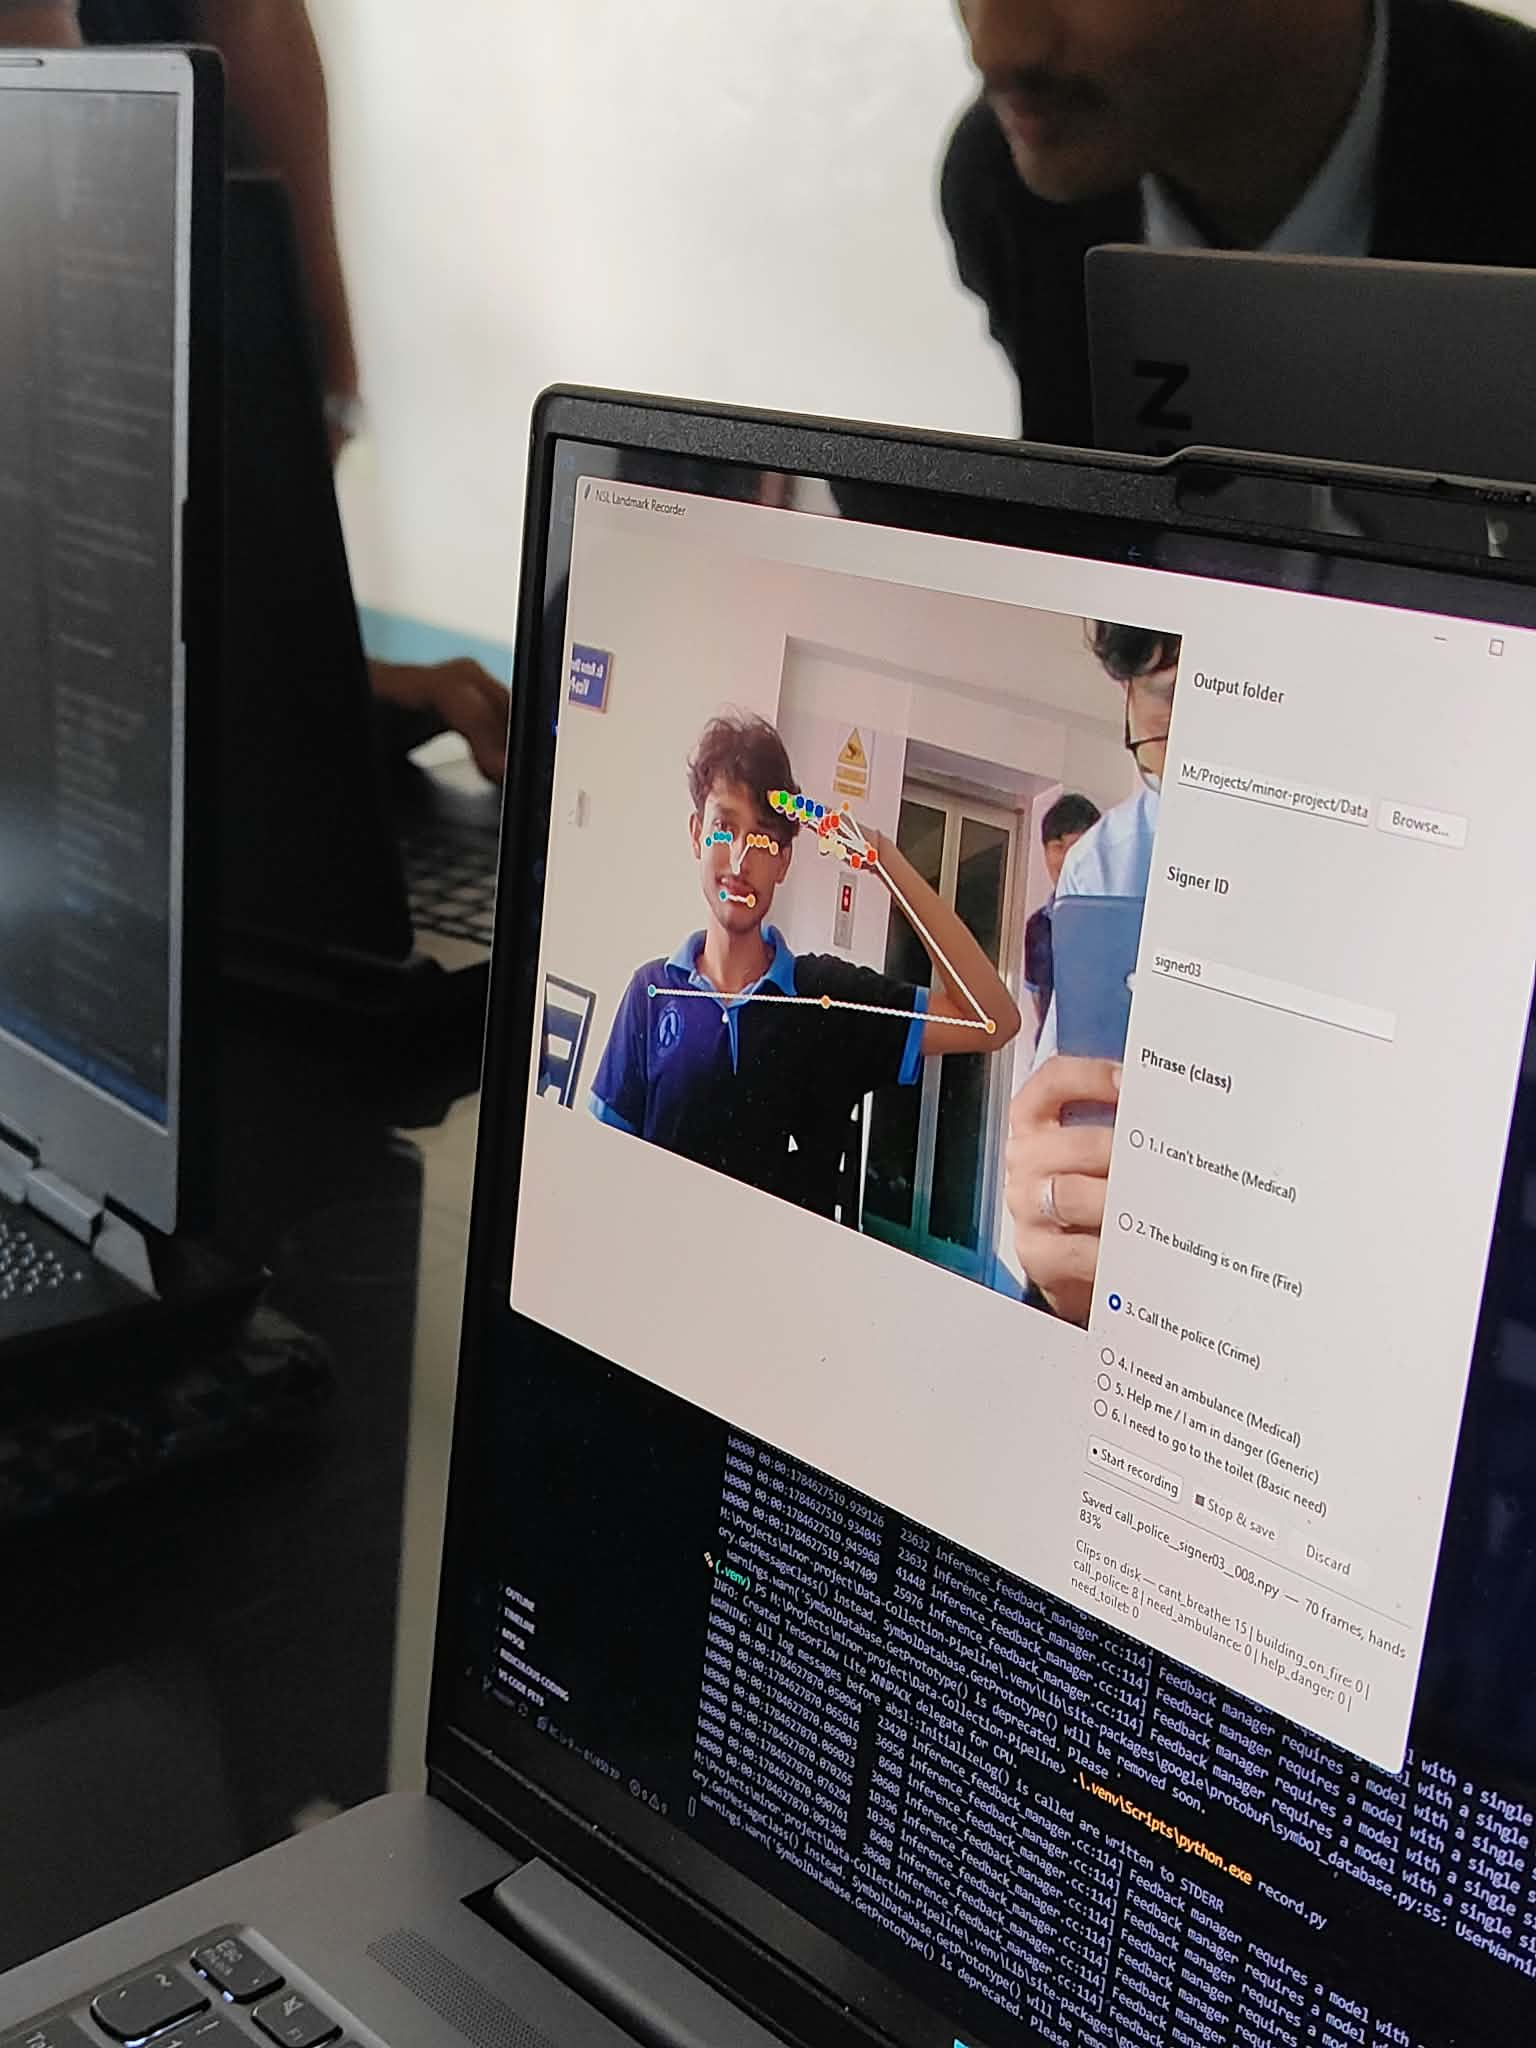
\includegraphics[width=0.88\textwidth]{img/recorder1.jpg}
    \caption{A signer recording the \textit{Call the police} phrase, showing live pose and hand landmark overlays alongside the signer identity and phrase selection}
    \label{fig:recorder-a}
\end{figure}

\begin{figure}[H]
    \centering
    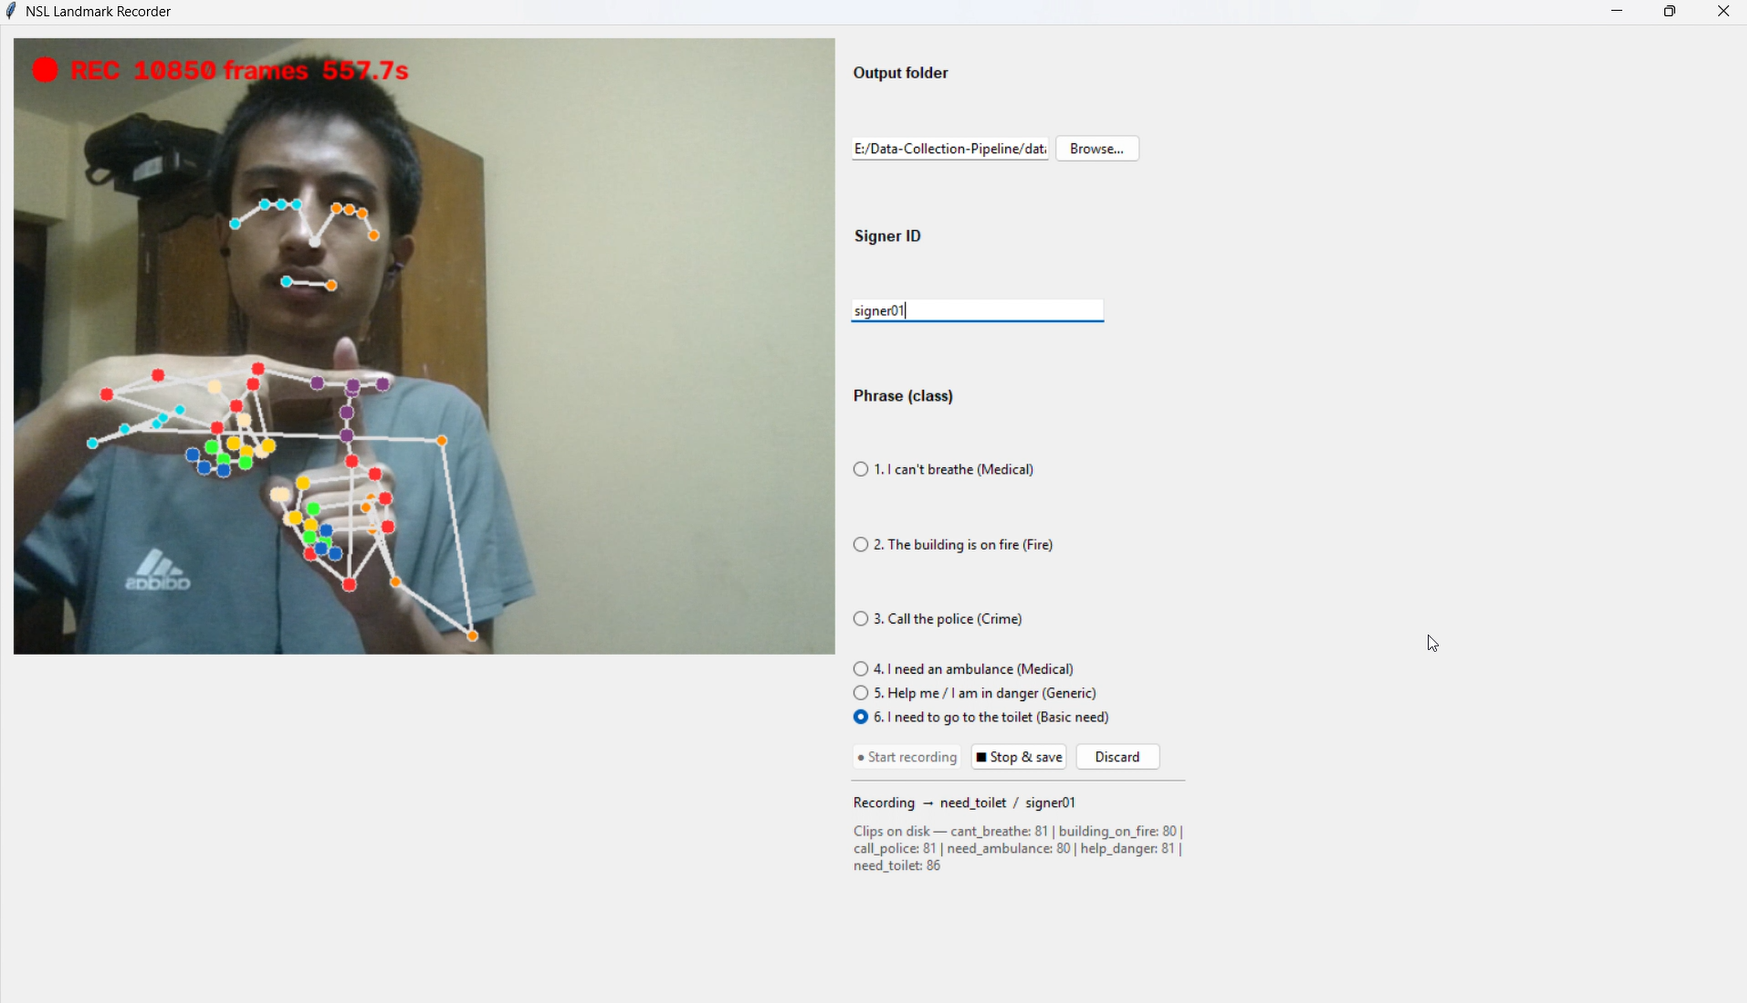
\includegraphics[width=0.88\textwidth]{img/recorder2.png}
    \caption{The recorder during an active recording, showing hand landmarks in detail and the running per-class clip counts on disk}
    \label{fig:recorder-b}
\end{figure}

% ================= Appendix C =================
\chapter{Dataset Organisation}
\label{app:dataorg}

The eight signers recorded independently on separate machines. Contributions were merged through a shared Git repository instead of by hand, which gave a reviewable history of what each signer added and caught duplicate and misnamed clips before they entered the combined dataset.

\begin{figure}[H]
    \centering
    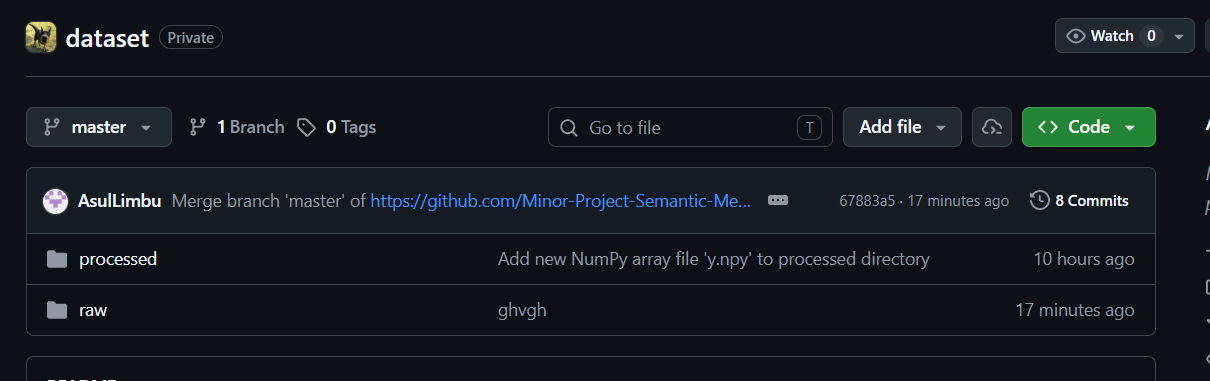
\includegraphics[width=0.88\textwidth]{img/repomerge1.png}
    \caption{The shared dataset repository, with raw and processed directories tracked separately and a commit history showing contributions merged from several signers}
    \label{fig:merge-repo}
\end{figure}

\begin{figure}[H]
    \centering
    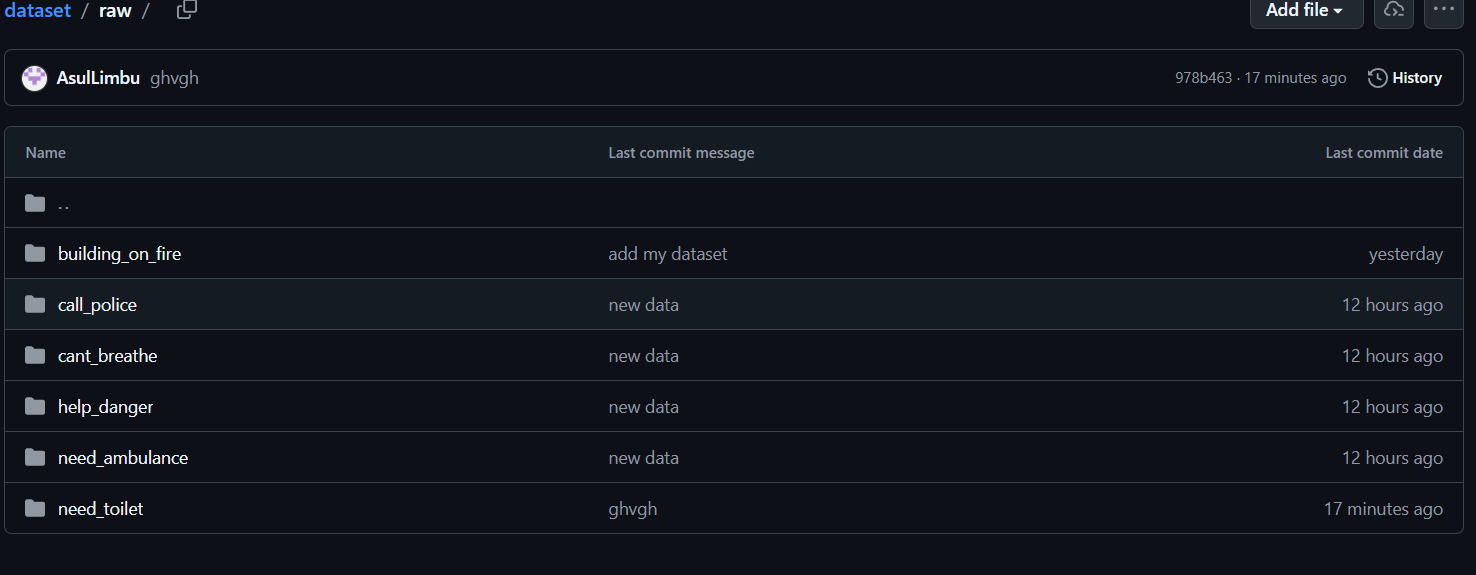
\includegraphics[width=0.88\textwidth]{img/repomerge2.png}
    \caption{The raw directory after merging, with one subfolder per phrase class holding the contributions of all signers}
    \label{fig:merge-raw}
\end{figure}

\begin{figure}[H]
    \centering
    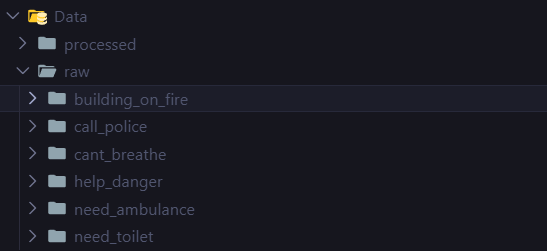
\includegraphics[width=0.5\textwidth]{img/rawdirs.png}
    \caption{Local directory layout: raw clips organised by phrase class, alongside the processed output directory}
    \label{fig:dirs-raw}
\end{figure}

\begin{figure}[H]
    \centering
    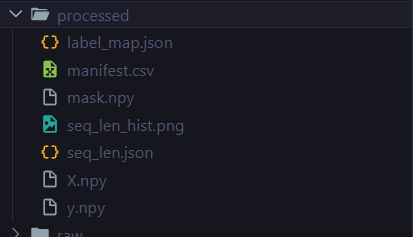
\includegraphics[width=0.42\textwidth]{img/processeddirs.png}
    \caption{Contents of the processed directory: the compiled tensors alongside the manifest and the sequence-length metadata}
    \label{fig:dirs-processed}
\end{figure}

% ================= Appendix D =================
\chapter{Sample Landmark Data}
\label{app:sampledata}

This appendix traces one clip through the preprocessing pipeline, to make the numeric effect of each step concrete. The clip is \texttt{call\_police\_\_signer01\_\_001.npy}, stored as a $(42, 225)$ array of 32-bit floats: 42 recorded frames, each holding one 225-value landmark vector.

\section{Feature Vector Layout}

\begin{table}[H]
    \centering
    \caption{Layout of the 225-value feature vector}
    \label{tab:featurelayout}
    \begin{tabular}{lccl}
        \toprule
        \textbf{Block} & \textbf{Indices} & \textbf{Values} & \textbf{Content} \\
        \midrule
        Pose        & 0 to 98    & 99 & 33 landmarks $\times\ (x, y, z)$ \\
        Left hand   & 99 to 161  & 63 & 21 landmarks $\times\ (x, y, z)$ \\
        Right hand  & 162 to 224 & 63 & 21 landmarks $\times\ (x, y, z)$ \\
        \midrule
        \textbf{Total} & & \textbf{225} & \\
        \bottomrule
    \end{tabular}
\end{table}

\section{Raw Values}

The first five pose landmarks of the clip's first frame, in the normalised image coordinates MediaPipe reports:

\begin{table}[H]
    \centering
    \caption{Raw pose landmarks 0 to 4, first frame}
    \label{tab:rawvalues}
    \begin{tabular}{cccc}
        \toprule
        \textbf{Landmark} & $x$ & $y$ & $z$ \\
        \midrule
        0 & 0.3683 & 0.3315 & $-$1.0291 \\
        1 & 0.3924 & 0.2687 & $-$0.9459 \\
        2 & 0.4069 & 0.2707 & $-$0.9461 \\
        3 & 0.4187 & 0.2732 & $-$0.9460 \\
        4 & 0.3420 & 0.2707 & $-$0.9640 \\
        \bottomrule
    \end{tabular}
\end{table}

\noindent Both hand blocks of this frame are entirely zero. The signer's hands had not yet entered the frame when recording began, MediaPipe reported no hand landmarks, and the recorder filled all 126 values with zeros instead of leaving them undefined.

\section{After Normalisation}

The same five landmarks after dual-anchor normalisation, now expressed relative to the shoulder midpoint and scaled by shoulder width:

\begin{table}[H]
    \centering
    \caption{Normalised pose landmarks 0 to 4, first frame}
    \label{tab:normvalues}
    \begin{tabular}{cccc}
        \toprule
        \textbf{Landmark} & $x$ & $y$ & $z$ \\
        \midrule
        0 & $-$0.0054 & $-$0.7148 & $-$1.6152 \\
        1 & 0.0463 & $-$0.8491 & $-$1.4370 \\
        2 & 0.0772 & $-$0.8449 & $-$1.4374 \\
        3 & 0.1025 & $-$0.8396 & $-$1.4374 \\
        4 & $-$0.0617 & $-$0.8449 & $-$1.4758 \\
        \bottomrule
    \end{tabular}
\end{table}

\noindent The $x$ coordinates now sit around zero instead of around 0.37, because the origin has moved to the midpoint of the shoulders. The zero hand blocks remain exactly zero, since both normalisation formulas map a zero input to a zero output.

\section{After Length Standardisation}

The clip has 42 frames, fewer than the sequence length of 146, so it is zero-padded at the end. The result is a $(146, 225)$ array in which the first 42 frames are real and the remaining 104 are zero, with a boolean mask recording which is which. The final frame of the standardised clip is entirely zero, confirming that padding stays distinguishable from signal and that the masking layer will skip it.

% ================= Appendix E =================
\chapter{Client Interface}
\label{app:ui}

The Android client presents one of two outcomes for every recognition attempt: an accepted phrase, which is displayed and spoken, or a low-confidence result, which is reported without being spoken. A row of indicators below the camera preview reports what the server observed for each frame, so a failure during use can be attributed instead of guessed at.

\fillin{Insert client screenshots here: the accepted and low-confidence result states, the telemetry indicator row, and the server configuration screen.}

% ================= Appendix F =================
\chapter{Server Interface}
\label{app:protocol}

The inference server exposes the endpoints in Table~\ref{tab:endpoints}. The streaming endpoint is the path the client uses; the two prediction endpoints exist so that the server can be checked against the offline pipeline without needing a phone.

\begin{table}[H]
    \centering
    \caption{Server endpoints}
    \label{tab:endpoints}
    \small
    \begin{tabular}{|l|l|c|p{6.1cm}|}
        \hline
        \textbf{Method} & \textbf{Path} & \textbf{Key} & \textbf{Purpose} \\
        \hline
        GET  & \texttt{/health}            & no  & Backend, class list, thresholds, target frame rate \\
        \hline
        GET  & \texttt{/classes}           & yes & Class keys and display labels \\
        \hline
        POST & \texttt{/predict/landmarks} & yes & A clip supplied as JSON, for verification \\
        \hline
        POST & \texttt{/predict/npy}       & yes & The same clip as raw array bytes \\
        \hline
        WS   & \texttt{/ws/stream}         & yes & Live frames to a decision, the path the client uses \\
        \hline
    \end{tabular}
\end{table}

\noindent The health endpoint is deliberately unauthenticated so that container health checks and the client's reachability test keep working when a key is configured. Every other endpoint requires the key, compared with a constant-time function so that a wrong key cannot be narrowed down by timing the response.

\begin{table}[H]
    \centering
    \caption{Messages on the streaming endpoint}
    \label{tab:wsmessages}
    \small
    \begin{tabular}{|l|l|p{7.3cm}|}
        \hline
        \textbf{Direction} & \textbf{Message} & \textbf{Meaning} \\
        \hline
        Server & \texttt{ready}     & Session established; carries the target frame rate and class list \\
        \hline
        Client & binary frame       & One JPEG frame \\
        \hline
        Server & \texttt{ack}       & Whether the frame was kept, the running frame count, and whether pose and hands were detected \\
        \hline
        Client & \texttt{done}      & Signing has finished; produce a decision \\
        \hline
        Server & \texttt{result}    & Status, phrase, confidence, and the three most probable classes \\
        \hline
        Client & \texttt{reset}     & Discard the current clip and start again \\
        \hline
        Client & \texttt{ping}      & Keepalive, sent while idle between signs \\
        \hline
    \end{tabular}
\end{table}


\end{document}